%&latex

\documentclass{WileySev}
%\usepackage{standalone}
%\usepackage{epstopdf}
%%%%%%%%%%%%%%%%%%%%%%%%%%%%%%%%%%%%%%%%%%%%%%%%%%%%%%%%%%%%%%%%
%% Post Script Font File

% For PostScript text
% If you have font problems, you may edit the w-bookps.sty file
% to customize the font names to match those on your system.

\usepackage{w-bookps}

%%%%%%%
%% For times math: However, this package disables bold math (!)
%% \mathbf{x} will still work, but you will not have bold math
%% in section heads or chapter titles. If you don't use math
%% in those environments, mathptmx might be a good choice.

% \usepackage{mathptmx}


%%%%%%%%%%%%%%%%%%%%%%%%%%%%%%%%%%%%%%%%%%%%%%%%%%%%%%%%%%%%%%%%
%% Graphicx.sty for Including PostScript .eps files

\usepackage{graphicx}

%%%%%%%%%%%%%%%%%%%%%%%%%%%%%%%%%%%%%%%%%%%%%%%%%%%%%%%%%%%%%%%%
%% Other packages you might want to use:

% for chapter bibliography made with BibTeX
% \usepackage{chapterbib}

% for multiple indices
% \usepackage{multind}

% for answers to problems
% \usepackage{answers}

%%%%%%%%%%%%%%%%%%%%%%%%%%%%%%%%%%%%%%%%%%%%%%%%%%%%%%%%%%%%%%%%
%% Change options here if you want:
%%
%% How many levels of section head would you like numbered?
%% 0= no section numbers, 1= section, 2= subsection, 3= subsubsection
%%==>>
\setcounter{secnumdepth}{3}

%% How many levels of section head would you like to appear in the
%% Table of Contents?
%% 0= chapter titles, 1= section titles, 2= subsection titles, 
%% 3= subsubsection titles.
%%==>>
\setcounter{tocdepth}{2}

%% Cropmarks? good for final page makeup
%% \docropmarks %% turn cropmarks on

%%%%%%%%%%%%%%%%%%%%%%%%%%%%%%%%%%%%%%%%%%%%%%%%%%%%%%%%%%%%%%%%
%% DRAFT
%
% Uncomment to get double spacing between lines, current date and time
% printed at bottom of page.
% \draft
% (If you want to keep tables from becoming double spaced also uncomment
% this):
% \renewcommand{\arraystretch}{0.6}

%% MY MACRO %%
\usepackage{amsmath,amssymb}
\newcommand{\ds}{\displaystyle}
\usepackage{answers}
\newenvironment{solution}{\noindent \small \textbf{Solution: }}{\qed}
\newcommand{\tends}{\rightarrow}
\newcommand{\pd}[2]{\displaystyle \frac{\partial #1}{\partial #2}}
\newcommand{\Z}{Z}
\newcommand{\W}{W}
\newcommand{\ncr}[2]{^{#1}C_{#2}}
\newcommand{\pdn}[3]{\displaystyle \frac{\partial ^{#3} #1}{\partial #2 ^{#3}}}
\newcommand{\pdxy}[3]{\displaystyle \frac{\partial ^{2} #1}{\partial #3 \partial #2 }}
\newcommand{\e}{e}
\usepackage[pdf]{pstricks}

%\theoremstyle{definition}
\newtheorem{definition}{Definition}[chapter]

%%%%%%%%%%%%%%%%%%%%%%%%%%%%%%

\begin{document}

%%%%%%%%%%%%%%%%%%%%%%%%%%%%%%%%%%%%%%%%%%%%%%%%%%%%%%%%%%%%%%%%
%% Title Pages
%%
%% Wiley will provide title and copyright page, but you can make
%% your own titlepages if you'd like anyway

%% Setting up title pages, type in the appropriate names here:
\booktitle{Complex Variables}
%\subtitle{Complex Analysis}

\author{Amit K. Awasthi \\
\affil{Gautam Buddha University}
}
%or
%\authors{}

%% \\ will start a new line.
%% You may add \affil{} for affiliation, ie,
%\authors{Robert M. Groves\\
%\affil{Universitat de les Illes Balears}
%Floyd J. Fowler, Jr.\\
%\affil{University of New Mexico}
%}

%% Print Half Title and Title Page:
\halftitlepage
\titlepage


%%%%%%%%%%%%%%%%%%%%%%%%%%%%%%%%%%%%%%%%%%%%%%%%%%%%%%%%%%%%%%%%
%% Off Print Info

%% Add your info here:
\offprintinfo{Complex Variables, 1st Edition}{Amit K Awasthi}

%% Can use \\ if title, and edition are too wide, ie,
%% \offprintinfo{Survey Methodology,\\ Second Edition}{Robert M. Groves}


%%%%%%%%%%%%%%%%%%%%%%%%%%%%%%%%%%%%%%%%%%%%%%%%%%%%%%%%%%%%%%%%
%% Copyright Page
\begin{copyrightpage}{2014}%
Complex Variables.%
\end{copyrightpage}%
% Note, you must use \ to start indented lines, ie,
% 
% \begin{copyrightpage}{2004}
% Survey Methodology / Robert M. Groves . . . [et al.].
% \       p. cm.---(Wiley series in survey methodology)
% \    ``Wiley-Interscience."
% \    Includes bibliographical references and index.
% \    ISBN 0-471-48348-6 (pbk.)
% \    1. Surveys---Methodology.  2. Social 
% \  sciences---Research---Statistical methods.  I. Groves, Robert M.  II. %
% Series.\\

% HA31.2.S873 2004
% 001.4'33---dc22                                             2004044064
% \end{copyrightpage}

%%%%%%%%%%%%%%%%%%%%%%%%%%%%%%%%%%%%%%%%%%%%%%%%%%%%%%%%%%%%%%%%
%% Frontmatter >>>>>>>>>>>>>>>>

%%%%%%%%%%%%%%%%%%%%%%%%%%%%%%%%%%%%%%%%%%%%%%%%%%%%%%%%%%%%%%%%
%% Only Dedication (optional) 
%% or Contributor Page for edited books
%% before \tableofcontents

\dedication{-}

% ie,
%\dedication{To my parents}

%%%%%%%%%%%%%%%%%%%%%%%%%%%%%%%%%%%%%%%%%%%%%%%%%%%%%%%%%%%%%%%%
%  Contributors Page for Edited Book
%%%%%%%%%%%%%%%%%%%%%%%%%%%%%%%%%%%%%%%%%%%%%%%%%%%%%%%%%%%%%%%%

% If your book has chapters written by different authors,
% you'll need a Contributors page.

% Use \begin{contributors}...\end{contributors} and
% then enter each author with the \name{} command, followed
% by the affiliation information.

% \begin{contributors}
% \name{Masayki Abe,} Fujitsu Laboratories Ltd., Fujitsu Limited, Atsugi,
% Japan

% \name{L. A. Akers,} Center for Solid State Electronics Research, Arizona
% State University, Tempe, Arizona

% \name{G. H. Bernstein,} Department of Electrical and
% Computer Engineering, University of Notre Dame, Notre Dame, South Bend, 
% Indiana; formerly of
% Center for Solid State Electronics Research, Arizona
% State University, Tempe, Arizona 
% \end{contributors}

%%%%%%%%%%%%%%%%%%%%%%%%%%%%%%%%%%%%%%%%%%%%%%%%%%%%%%%%%%%%%%%%
\contentsinbrief %optional
\tableofcontents
% \listoffigures %optional
% \listoftables  %optional

%%%%%%%%%%%%%%%%%%%%%%%%%%%%%%%%%%%%%%%%%%%%%%%%%%%%%%%%%%%%%%%%
% Optional Foreword:

%\begin{foreword}
%text
%\end{foreword}

%%%%%%%%%%%%%%%%%%%%%%%%%%%%%%%%%%%%%%%%%%%%%%%%%%%%%%%%%%%%%%%%
% Optional Preface:

%\begin{preface}
% text
%\prefaceauthor{}
%\where{place\\
% date}
%\end{preface}

% ie,
% \begin{preface}
% This is an example preface.
% \prefaceauthor{R. K. Watts}
% \where{Durham, North Carolina\\
% September, 2004}

%%%%%%%%%%%%%%%%%%%%%%%%%%%%%%%%%%%%%%%%%%%%%%%%%%%%%%%%%%%%%%%%
% Optional Acknowledgments:

% \acknowledgments
% acknowledgment text
% \authorinitials{} % ie, I. R. S.


%%%%%%%%%%%%%%%%%%%%%%%%%%%%%%%%
%% Glossary Type of Environment:

% \begin{glossary}
% \term{<term>}{<description>}
% \end{glossary}

%%%%%%%%%%%%%%%%%%%%%%%%%%%%%%%%
% \begin{acronyms} 
% \acro{<term>}{<description>}
% \end{acronyms}

%%%%%%%%%%%%%%%%%%%%%%%%%%%%%%%%
%% In symbols environment <term> is expected to be in math mode; 
%% if not in math mode, use \term{\hbox{<term>}}

% \begin{symbols}
% \term{<math term>}{<description>}
% \term{\hbox{<non math term>}}Box used when not using a math symbol.
% \end{symbols}

%%%%%%%%%%%%%%%%%%%%%%%%%%%%%%%%
% \begin{introduction}
%\introauthor{<name>}{<affil>}
% Introduction text...
% \end{introduction}

%%%%%%%%%%%%%%%%%%%%%%%%%%%%%%%%%%%%%%%%%%%%%%%%%%%%%%%%%%%%%%%%
%% End for Front Matter, Beginning of text of book  >>>>>>>>>>>

%% Short version of title without \\ may be written in sq. brackets:

%% Optional Part :
%%%%%%%%%%%%%%%%%%%%%%%%%%%%%%%%%%%%%%%%%%%%%%%%%%%%%\part[Submicron Semiconductor Manufacture]
%%%%%%%%%%%%%%%%%%%%%%%%%%%%%%%%%%%%%%%%%%%%%%%%%%%%%{Submicron Semiconductor\\ Manufacture}

\chapter[Complex Numbers]
{Complex Numbers}
\section{Complex Numbers}
A complex number is a number of the form
\begin{equation}
z = a + i b
\label{zrect}
\end{equation}
where the imaginary unit is defined as
\footnote{In electrical engineering,
a lower case $i$ represents a time-dependent current, so it is
their convention to use the symbol $j$ in place of $i$.}
\begin{equation}
i = \sqrt{-1}
\label{idef}
\end{equation}
and $a$ is the real part of $z$, written $a = Re(z)$, and $b$ is the 
imaginary part of $z$, written $b = Im(z)$.     $a$ and
$b$ are real numbers. 

Complex numbers have real and imaginary parts.
However, if a number has no real part, then it is called
`pure imaginary'.


It may be easily verified 
from Eq. (\ref{idef}) that $i^2 = -1$, and that
\begin{equation}
\frac{1}{i} = -i
\end{equation}

\section{The Complex Plane}
A complex number can be visualized in a
two-dimensional number line, known as an 
Argand diagram, or the complex plane
as shown in Fig. \ref{argand}.
\begin{figure}
\begin{center}
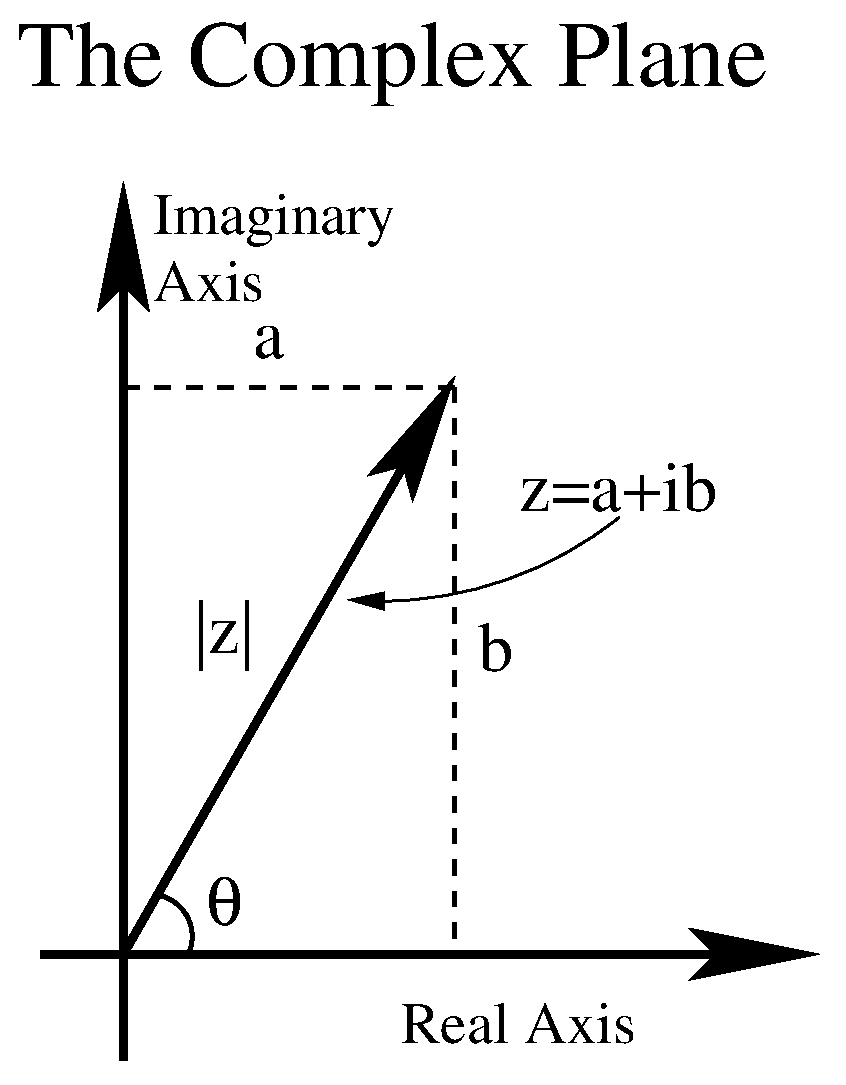
\includegraphics[width=5cm,height=5cm]{images/argand.eps}
\caption[The Complex Plane]{A complex number is easily visualized as
a "phasor" in the complex plane.}
\label{argand}
\end{center}
\end{figure}
The complex plane replaces the number line as a visualization
tool for real numbers.  However, rather than plot points
in the complex plane, it is conventional to represent
a complex number as a vector in the complex plane.  Instead
of calling them complexified vectors, they are referred to
as ``phasors.''  Note 
that because the visualization
is 2-dimensional, a polar form for complex numbers is suggested.
This is discussed below.%  

As an addition side note about the 
complex plane, complex analysis can be used to study
improper real integrals that couldn't otherwise be
solved.  Basically, for an integral that extends from
$-\infty$ to $\infty$, instead of integrating over
the real number line, one may perform a closed path line
integral that includes the real number line and a semicircle
of radius $R$, which is allowed to approach $\infty$.
The residue theorem relates the closed loop integral
to a real value.  However, it can be shown that the
integral over the infinite semicircle approaches zero,
and our integral of interest is obtained.

\section{Complex Magnitude}
From Fig. \ref{argand}, it can be easily seen (using the Pythagorean theorem) 
that the magnitude, or length, of the vector representing
a complex number is
\begin{equation}
|z| = \sqrt{a^2 + b^2}
\end{equation}
Thus, the complex magnitude is the 
square root of the sum of the squares of the real 
and imaginary parts of the complex number.
This definition generalizes the absolute value
function of a real number.

\section{Complex Conjugate}
The complex conjugate of a complex number $z$, is denoted
$\bar{z}$, and is defined
\[
\bar{z} = a - i b
\label{zconjrect}
\]
We may think of the conjugation process as
``replacing $i$ with $-i$.''

Where would the vector $\bar{z}$ fit on the complex plane in Fig \ref{argand}?

\begin{example}[Complex Conjugate]
Prove that $\bar{z}z = |z|^2$.
\end{example}
\begin{proof}
\begin{eqnarray*}
\bar{z}z &=& (a - ib)(a+ib) \\
&=& a^2 + b^2 \\
&=& (a^2 + b^2)^{1/2} (a^2 + b^2)^{1/2} \\
&=& \samepage |z|^2
\end{eqnarray*}
\end{proof}
Note that $\bar{z}z$ is real and positive.  A quotient of complex numbers can 
be written separated 
into real and imaginary parts using the above conjugate relation
as shown in the next example.

\begin{example}
\textbf{Complex Fractions}\\
Separate the complex number $z = \frac {3-i4}{5+i12}$
into real and imaginary parts.
\end{example}
\begin{proof}
The solution involves the well known rationalizing 
the denominator technique of multiplying the top and bottom of the quotient 
by the conjugate of the denominator.

\begin{eqnarray*}
z &=& \frac {3-i4}{5+i12} \\
  &=& \frac {3-i4}{5+i12} \frac {5-i12}{5-i12}  \\
  &=& \frac {(15-48)+i(-20-36)}{13} \\
  &=& - \frac {33+i56}{13} 
\end{eqnarray*}
\end{proof}
It may be noted that $|\bar{z}| = |z|$.  Also, the conjugate of a product 
is a product of conjugates so that $\overline{(uv)} = \bar{u} \bar{v}$.  Similarly, 
the conjugate of a sum is the sum of conjugates so that 
$\overline{(u + v)} = \bar{u} + \bar{v}$.
Finally, the conjugate of a conjugate is the function itself, i.e.
$\overline{(\overline{z})} = z$.  Put another way, complex conjugation ``toggles.''

\begin{example}
Consider the function $f(z) = 3z^2 +(2+i7)z + i6$ where $z$ is 
a complex variable. \\
\indent
a)      What is the conjugate of  the function, $f^*(z)$? \\
\indent
b)      What is $f(\bar{z})$? \\
\indent
c)      What is $f^*(\bar{z})$? \\
\end{example}

\begin{proof}
Following the simple steps:
\begin{eqnarray*}
a)  f^*(z) &=& [3z^2 + (2+i7)z + i6]^* \\
           &=& (3z^2)^* + [(2+i7)z]^* + (i6)^* \\
           &=& 3z^{*2} +[(2+i7)^*\bar{z}] +i^*6^* \\
           &=& 3z^{*2} + (2-i7)\bar{z} - i6 \\
b)  f(\bar{z}) &=& 3z^{*2} +(2+i7)\bar{z} + i6 \\ 
c)  f^*(\bar{z}) &=& 3z^2 + (2-i7)z - i6 \\
\end{eqnarray*}
\end{proof}


\section{Polar Form of a Complex Number}
Let $r$ be the magnitude of  the complex number 
$z$, and let $\theta$ be the angle that the line from origin to the complex number $z$ makes with the positive $x$-axis. Here, note that $\theta$ is
not defined if $z=0$. The complex number $z$
can be expressed in terms of a magnitude, $r$,  and the  angle, $\theta$, as
\begin{equation}
z = r (cos \theta  + i sin\theta)
\label{zpolar2}
\end{equation}
 Due to Euler, we have a well known result
\begin{equation}
e^{i \theta} = cos(\theta ) + i sin(\theta )
\label{euler}
\end{equation}
This is one of the most powerful results in
all of mathematics.  Basically, all of the
trignometric identities can be derived from it.
Substituting the Euler Relation (Eq 
\ref{euler}) into (Eq \ref{zpolar2}) yields
\begin{equation}
z = r e^{i \theta}
\label{zpolar}
\end{equation}
Thus, a complex number can be thought of as having two forms:  
a rectangular form (Eq. \ref{zrect}) and a polar form (Eq. \ref{zpolar}).  

The complex conjugate of Eq. (\ref{euler}) is
\begin{equation}
e^{-i \theta}= cos(\theta ) - i sin(\theta )
\label{eulerconj}
\end{equation}
Adding Eqs. (\ref{euler}) and (\ref{eulerconj}) and dividing by 2 yields the 
important result
\begin{equation}
cos(\theta ) = \frac {e^{i \theta} + e^{-i \theta}}{2}
\label{cos}
\end{equation}
Similarly,
\begin{equation}
sin( \theta ) = \frac {e^{i \theta} - e^{-i \theta}}{2i}
\label{sin}
\end{equation}
While the Euler relation is the most important result
here, these two closely follow.  While extremely useful,
it is also generally interesting that the sum of complex
functions yields a real function.

In the polar form the conjugate of $z$ is
\begin{equation}
\bar{z} = r e^{-i \theta}
\label{zconjpolar}
\end{equation}
Using the polar form, the result from Example A.1 becomes 
transparent.

\begin{example}
\textbf{The Euler Relation}\\
Use Euler's identity to derive the formula for the cos of the 
sum of two angles.
\end{example}
\begin{proof}
If $Re \{ \}$ represents an operator which takes the real
part of a complex number or function, then from
Eq. (\ref{cos})
\begin{eqnarray*}
cos(a + b) &=& Re \{ e^{i(a + b)} \} \\
&=& Re \{ e^{ia} e^{ib} \} \\
&=& Re \{ [cos(a) + i sin(a)] [cos(b) + i sin(b)] \} \\
&=& Re \{ [cos(a) cos(b) - sin(a) sin(b)] + i[sin(a) cos(b) + cos(a) sin(b)] \} \\
&=& cos(a) cos(b) - sin(a) sin(b)
\end{eqnarray*}
Clearly the $sin(a+b)$ is also readily obtained.
\end{proof}

\section{Hyperbolic Sin and Cos}
It is clear that the $sin$ and $cos$ of a real number is
a real number, but what about the $sin$ and $cos$ of a 
number that is pure imaginary?
From Eqs. (\ref{cos}) and (\ref{sin}) it follows that the $sin$ and
$cos$ of a pure imaginary number is ... drumroll, please ... real!
This was the inspiration for defining hyberbolic $cos$ and $sin$.
They are defined by simply erasing the ``$i$'s'' in Eqs. (\ref{cos})
and (\ref{sin}):
\begin{equation}
cosh(\theta ) = \frac {e^{\theta} + e^{- \theta}}{2}
\end{equation}
\begin{equation}
sinh( \theta ) = \frac {e^{\theta} - e^{- \theta}}{2}
\end{equation}
Of course, once you have $sinh$ and $cosh$, you can define
$tanh$, $coth$, $arcsinh$, ...  In addition, there are 
hyberbolic trigonmetric identities.  For example, by looking
at the above equations, you should be able to confirm
(without pencil and paper!) that
\begin{equation}
cosh^2(x) - sinh^2(x) = 1
\end{equation}
The switching from the variable $\theta$ to $x$ was intentional.
The argument of a sinusoid is an angle (in radians), while
the argument of a hyberbolic sinusoid is not (it's dimensionless).

\section{Converting Between Polar and Rectangular Forms}
A complex number written in polar form may be converted to 
rectangular form by the relations
\begin{equation}
a = A cos(\theta )
\end{equation}
\begin{equation}
b = A sin(\theta )
\end{equation}
These are immediately obtained by substituting the Euler relation
into the polar form of a complex number.
Conversely, these equations may be inverted, and a complex 
number written in rectangular form may be converted to polar 
form by the relations
\begin{equation}
A = \sqrt{a^2 + b^2}
\end{equation}
\begin{equation}
\theta = tan^{-1}(b/a)
\end{equation}
These four formulas are identical to normal polar-to-Cartesian
and vice-versa conversions.  Quite often in complex number
calculations, one switches between the two forms.

\section{Powers and Roots of Complex Numbers}
A most logical way to continuing our study of complex numbers
would be to look at the $sin$ and $cos$ of a complex number,
the exponential function of a complex number, powers and
roots of complex numbers...  Basically, separate any elementary 
function\footnote {and special functions such as Bessel
functions too!} of a complex number into real and imaginary parts.
The $sin$, $cos$, and exponential functions are easy, and
left to the reader as an exercise.  Here we consider powers
and roots of complex numbers.

As a first step in this method is to write your complex number
in polar form.  With this done, the power of a complex number
is easily calculated:
\begin{equation}
z^n = A^n e^{in \theta}
\end{equation}
If desired (or required), one would then convert this
back to the rectangular form.  Solving problems involving
complex numbers and functions often involves switching
back and forth between rectangular and polar form.

Roots of complex numbers may be obtained in a nearly
identical manner:
\begin{equation}
z^{1/n} = A^{1/n} e^{i\theta /n}
\end{equation}
It is interested and inciteful to interpret these
results graphically.  The angle is reduced by a factor
of $1/n$ and the magnitude is affected in the same way
as the square root of a real number is.  For a complex
number of unit magnitude, a plot of a complex number
with three of its roots are shown.
\begin{figure}
\begin{center}
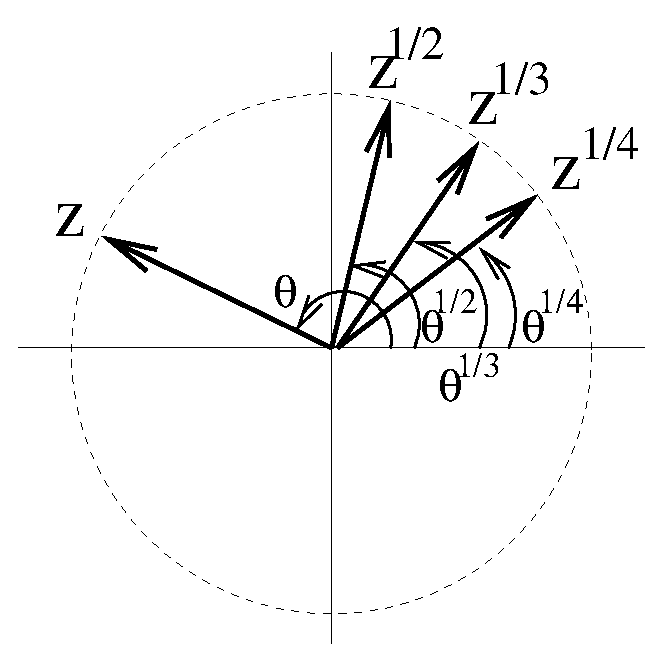
\includegraphics[width=7cm,height=7cm]{images/root.eps}
\caption[Roots of Complex numbers]{The $n$th root of a
complex number is an angle which 1/$n$th the original number.}
\end{center}
\end{figure}
At times it is useful to have the formula for a root of a complex 
number in rectangular form. While this can't be done in general, 
the square root is tractable:
\begin{equation}
\sqrt{a+ib} = 
\sqrt{\frac{\sqrt{a^2 + b^2} +a}{2}} +isgn(b)
\sqrt{\frac{\sqrt{a^2 + b^2} -a}{2}}
\end{equation}
where $sgn(b)$ is the signum function, which is also known
as the sign of $b$.  The signum function is generally 
defined as $b/|b|$.  We define $sgn(0)$ to be unity.

\section{The Problem that ``Can't Be Done''}
In pre-calculus and even in calculus, you may have been told
that calculating the $arccos$ of a number greater than 1
can't be done.  Since the $cos$ function oscillates between
-1 and 1, calculating $arccos(3)$ would be ``difficult.''
When I ask my calculator to calculate $arccos(3)$, it says
``Error 0.''

Of course the calculator and the early math courses are
restricting themselves to the real number system.\footnote{Your 
calculator may not have this restriction.}
The $arccos(3)$, for example, is just a complex number.
In fact, it is pure imaginary, as we will now show.


\begin{example}
\textbf{Inverse Trig Functions}\\
Calculate $arccos(3)$.
\end{example}

\begin{proof}
let 
\begin{equation}
y uiv arccos(3)
\end{equation}, then $cos(y) = 3$.
But from the Euler Relation, the $cos$ function
can be written as a sum of complex exponentials:
\begin{equation}A
\frac {e^{iy} + e^{-iy}}{2} = 3
\end{equation}
A
Multiplying both sides by $2e^{iy}$, and moving
all terms to the left hand side of the equation
results in
\begin{equation}A
{\left ( e^{iy} \right ) }^2 - 6e^{iy} +1=0
\end{equation}A
which is a quadratic equation in $e^{iy}$.  The
solutions are
\begin{equation}A
e^{iy}=3 \pm 2 \sqrt{2}
\end{equation}A
Taking the natural log of both sides and multiplying by
$-i$ results in
\begin{equation}A
y = -i ln(3 \pm 2 \sqrt{2})
\end{equation}A
\end{proof}

%%%%%%%%%%%%%%%%%%%%%%%%%%%%%%%%%%%%%%%%%%%%%%%%%%%%%%%%
%%%%%%%%%%%%%%%%%%%%%%%%%%%%%%%%%%%%%%%%%%%%%%%%%%%%%%%%

\section{PROBLEMS}

\begin{problems}
Separate the following into real and imaginary parts:\\
a)      $\frac{3+i4}{5+i7}$\\
b)      $(3+i4) +i(4+i5) + (2+i3)(4+i5)^2$\\
c)      $tan(3+i4)$\\
d)      $e^{3+i4}$\\
e)      $\sqrt{1+i2}$\\
f)      $ln(3+i4)$\\
g)      $sin^{-1} (3)$\\
h)      $i^i$\\
        Hint: $i$ can be thought of as a complex number in rectangular form.\\
i)      There are an infinite number of values for $i^i$, what are they?\\
        Hint: $e^{i \theta} = e^{i( \theta + 2n \pi )}$\\
\end{problems}

\begin{problems}
Consider a series AC electrical circuit with two resistors
and a capacitor.
\begin{figure}[h]
\begin{center}
\includegraphics[width=7cm,height=3cm]{images/RRC1.eps}
\caption[RC Circuit]{A simple AC circuit.}
\end{center}
\end{figure}
The output complex voltage is related to the input complex voltage by 
the voltage divider law
\[
{\hat{V}}_{out} = \frac{R_2}{R_1 + R_2 -i/(\omega C)} {\hat{V}}_{in}
\]
If $R_1 = 100 \Omega $, $R_2= 200 \Omega $, $C = 50 {\mu}F$, and 
$\omega = 2 \pi (60)$ cycles/s, and ${\hat{V}}_{in} = 100 V$, 
then what is the \\

a)      magnitude of the output voltage,\\
b)      phase of the output voltage.\\
c)      plot $| {\hat{V}}_{out} / {\hat{V}}_{in} |$ as a function 
of differents $\omega$'s.
\end{problems}

\begin{problems}
If $\Psi$ is the wave function from the Schr\"{o}dinger equation, then
the probability density of finding a particle at a particular
place is given by $P(x) = \Psi ^* \Psi$.  Suppose that you
have solved the Schr\"{o}dinger equation for a given potential
functions, and you find that
\[
\Psi (x) = \frac{p}{1+qx^2}
\]
where $p=p_r +i p_i$, $q=q_r + iq_i$ are complex constants, and
$P=p^*p$, and $Q=q^*q$.
Compute the probability density distribution in this case.
(Note: $x$ is a real variable).
\end{problems}


\begin{problems}
One problem of interest is the writing of
the $n^{th}$ power of $cos$ into a Fourier series.
Using trigonometric identities it is generally difficult to
prove that
\[
cos^m(\omega t) = \frac{1}{2^m}
\sum_{k=0}^m \frac{m!}{k!(m-k)!} cos[(m-2k) \omega t]
\]
Use the Euler relation to derive the above result\footnote {As the
student may be aware, the
binomial theorem is $(a+b)^m = \sum_{k=0}^m \frac{m!}{k!(m-k)!} 
a^k b^{m-k}$}.
\end{problems}

\begin{problems}
Plot the following phasors tail-to-tip on a piece of graph
paper:\\
\begin{eqnarray*}
2 - \sqrt{29}e^{-i tan^{-1}(5/2)} + (\sqrt{34}/5)e^{+i tan^{-1}(3/5)} -2 + 
(\sqrt{136}/5)e^{-i tan^{-1}(3/5)}
\end{eqnarray*}
\begin{eqnarray*}
- \sqrt{5}e^{-i tan^{-1}(2)} 
- \sqrt{5}e^{+i tan^{-1}(2)} 
+ (\sqrt{34}/5)e^{+i tan^{-1}(3/5)} -
(\sqrt{29}/5)e^{+i tan^{-1}(5/2)} +2
\end{eqnarray*}
Hints: 1)  Start near the bottom middle of your graph paper.
2)  The sum of the complex numbers is zero, so the last
phasor should end at the same place your first complex number
started.
\end{problems}
\begin{problems}
The complex propagation constant for an electromagnetic
wave propagating in a conductive medium can be obtained
from the formula
\begin{eqnarray*}
        {k_0}^2 & = &  {\omega}^2 \mu \epsilon - i \mu \sigma \omega \\
        & \equiv & (\beta_0 - i\alpha_0 )^2 
\end{eqnarray*}
where ${\beta}_0$ is the propagation constant and ${\alpha}_0$
is the loss per length.  
\begin{description}
        \item[a)] If the skin depth
                $\delta = 1/ {\alpha}_0$, then
                obtain an analytical expression for $\delta$ in terms of
                $\omega$, $\mu$, $\epsilon$, and $\sigma$.
        \item[b)] Simply you expression for 
                $\frac{\sigma}{\omega \epsilon} << 1$.
\end{description}
\end{problems}

\begin{problems}
Use the Euler Relation to derive the trigonometric identity for
the $sin$ of the sum of two different angles:  $sin(a+b)$.
\end{problems}

\begin{problems}
Often times books show a proof of Euler's Identity by
looking at the Taylor series expansion for $sin(x)$ and
$cos(x)$, comparing it to the expansion for $e^x$ and
saying ``Tada, it works!''  Here the goal is to 
$derive$ the Euler relation,
assuming that we know a little bit about differential
equations.  Put another way, we don't want to just show
that it happens to work, but that it $must$ work.
First, we consider the following differential
equation which represents simple harmonic motion such
as from a pendulum (small angles) or a spring:
\[
\frac{d^2y}{dt^2} + {\omega}^2 y(t) = 0
\]
Complete the following steps of the derivation:\\
\begin{description}
\item[a)]Show that $y(t)= a sin( \omega t) + b cos( \omega t)$
are solutions to the differential equation.
\item[b)]Apply the boundary conditions $y(0)=y_0$ and
$y^{\prime}(0) = y^{\prime}_0$ to this solution.
\item[c)]Show that $y(t)= A e^{i \omega t} + B e^{-i \omega t}$
are solutions to the differential equation.
\item[d)]Apply the boundary conditions $y(0)=y_0$ and
$y^{\prime}(0) = y^{\prime}_0$ to this solution.
\item[e)]Since the differential equation is second order, it
has only two independent solutions.  Thus coefficients of
the $y_0$ terms in the two equations must be equal to each
other.  Set them equal to each other, and solve for
$e^{i \omega t}$.
\end{description}
\end{problems}

\begin{problems}
Make separate plots of the following roots 
as phasors in the complex plane:\\
a)      $z^2 = 1$\\     
b)      $z^3 = 1$\\     
c)      $z^4 = 1$\\     
d)      $z^5 = 1$\\     
e)      $z^3 = \frac{1+i}{\sqrt{2}}$\\
\end{problems}



\chapter[Analytic Functions]
{Analytic Functions}
\input{complex/analytic}

\chapter[Complex Integration]{Complex Integration}
%\chapter{Complex Integration}\index{Complex integration}
\section{Integration in complex plain}
In case of real variable, the path of the integration of $\ds \int_a^b f(x)dx$ is always along the $x$-axis from $x=a$ to $x=b$. But in case of a complex function $f(z)$ the path of a complex function $f(z)$ the path of the definite integral $\ds \int_{\alpha}^{\beta} f(z)dz$ can be along any curve from $z=\alpha$ to $z=\beta$. 
\begin{example}
Evaluate $\ds \int_{0}^{2+i} \bar{z}^2 dz$ along the real axis from $z=0$ to $z=2$ and then along parallel to $y$-axis from $z=2$ to $z=2+i$.
\end{example}
\begin{solution}
\begin{align*}
	\int_{0}^{2+i} \bar{z}^2 dz		&= \int_{0}^{2+i} (x-iy)^2 (dx+idy)\\
																&= \int_{0}^{2+i} (x^2-y^2-2ixy) (dx+idy)\\
\end{align*}
\begin{figure}[ht]
  \begin{center}
\scalebox{0.7} % Change this value to rescale the drawing.
{
\begin{pspicture}(0,-1.08)(2.9934375,1.05)
\psline[linewidth=0.02cm,arrowsize=0.05291667cm 2.0,arrowlength=1.4,arrowinset=0.4]{<-}(0.2778125,1.04)(0.2778125,-0.74)
\psline[linewidth=0.02cm,arrowsize=0.05291667cm 2.0,arrowlength=1.4,arrowinset=0.4]{->}(0.2778125,-0.74)(2.7178125,-0.74)
\psline[linewidth=0.02cm,arrowsize=0.05291667cm 2.0,arrowlength=1.4,arrowinset=0.4]{->}(0.2778125,-0.74)(1.6978126,0.56)
\psline[linewidth=0.02cm,arrowsize=0.05291667cm 2.0,arrowlength=1.4,arrowinset=0.4]{<-}(1.6778125,0.58)(1.6778125,-0.74)
\usefont{T1}{ptm}{m}{n}
\rput(1.7167188,-0.93){z=2}
\usefont{T1}{ptm}{m}{n}
\rput(2.2298439,0.55){z=2+i}
\usefont{T1}{ptm}{m}{n}
\rput(2.8632812,-0.73){x}
\usefont{T1}{ptm}{m}{n}
\rput(0.085625,0.93){y}
\end{pspicture} 
}
\end{center}
\caption{}
\end{figure}
\paragraph{Along real axis from $z=0$ to $z=2$ (y=0)}:
\[y=0 \Rightarrow dy=0, dz = d(x+iy) = dx \]
\[z=0, y=0 \Rightarrow x=0\]
and
\[z=2, y=0 \Rightarrow x=2\]
\begin{align*}
	\int_{0}^{2+i} \bar{z}^2 dz		&= \int_{0}^{2} (x^2) (dx)\\
	&= \left[\frac{x^3}{3} \right]_0^2 = \frac{8}{3}\\
\end{align*}
\paragraph{Along parallel to $y$-axis from $z=2$ to $z=2+i$ (x=2)}
\[x=2 \Rightarrow dx=0, dz = d(x+iy) = idy\]
\[z=2, x=2 \Rightarrow y=0~~~~~and~~~~~z=2+i, x=2 \Rightarrow y=1\]
\begin{align*}
	\int_{0}^{2+i} \bar{z}^2 dz		&= \int_{0}^{1} (4-y^2-4iy) (i.dy)\\
	&= i \left[4y - \frac{y^3}{3} - 4i\frac{y^2}{2} \right]_0^1 =\left[\frac{11}{3}i + 2\right]\\
\end{align*}
$\ds \int_{0}^{2+i} \bar{z}^2 dz$ along the real axis from $z=0$ to $z=2$ then along parallel to $y$-axis from $z=2$ to $z=2+i$
\[= \frac{8}{3} +  \frac{11}{3}i + 2  = \frac{1}{3}(14+11i)\]
\end{solution}
\begin{problems}
\prob Find the value of the integral 
\[\int_0^{1+i}(x-y+ix^2)dz\]
\subprob Along the straight line from $z=0$ to $z=1+i$.
\begin{sol}\[\frac{1}{3}(i-1)\]\end{sol}
\subprob along the real axis from $z=0$ to $z=1$ and then along parallel to $y$-axis from $z=1$ to $z=1+i$.
\begin{sol}\[-\frac{1}{2}+\frac{5}{6}i\]\end{sol}
\prob Integrate $f(z) = x^2 + ixy$ from $A(1,1)$ to $B(2,8)$ along
\subprob the straight line $AB$
\begin{sol}
Equation of line $AB$
\[y=7x-6\]
Now 
\[\int f(z) dz  = \int (x^2 + ixy)(dx+idy)\]
substitute $y=7x-6$, $dy=7dx$, then on integrating
\[=\frac{1}{3}[-147+71i]\]
\end{sol}
\subprob the curve $C$, $x=t, ~y=t^3$.
\begin{sol}
Here
\[\int f(z) dz  = \int (x^2 + ixy)(dx+idy)\]
substitute $x=t,y=t^3$, $dx=dt\text{ and } dy=3t^2dt$, then on integrating with respect to $t$ from 1 to 2
\[=-\frac{1094}{21}+\frac{124}{5}i\]
\end{sol}

\prob Evaluate the integral $\ds \int_c (3y^2dx+2ydy)$, where $c$ is the circle $x^2+y^2=1$, counterclockwise from $(1,0)$ to $(0,1)$.
\begin{sol}
-1
\end{sol}
\end{problems}

\section{Cauchy's Integral Theorem}\index{Cauchy's Integral Theorem}
\begin{theorem}
If a function $f(z)$ is analytic and its derivative $f'(z)$ continuous at all points within and on a simple closed curve $c$, then $\ds \int_c f(z) dz = 0$.
\end{theorem}
\begin{proof}
Let $f(z)=u+iv$ and $z=x+iy$ and region enclosed by the curve $c$ be $R$, then
\begin{align*}
	\int_cf(z)dz 	&= \int_c(u+iv)(dx+idy) =  \int_c(udx-vdy) + i(vdx+udy)\\
								&= \int\int_R (-v_x - u_y)dxdy + i\int\int_R (u_x - v_y)dxdy\\
								\text{By Cauchy-Riemann equations,} \\
								&= \int\int_R (u_y - u_y)dxdy + i\int\int_R (u_x - u_x)dxdy =0
\end{align*}
\end{proof}
\begin{example}
Find the integral $\ds \int_c \frac{3z^2+7z+1}{z+1}dz$, where $c$ is the circle $\ds |z|=\frac{1}{2}$.
\end{example}
\begin{solution}
Poles of integrand are given by
$$z+1 = 0$$
That is, $z=-1$. Since given circle $|z|=\frac{1}{2}$, with centre $z=0$ and radius $1/2$ does not enclose $z=-1$. Thus it is obvious that the integrand is analytic everywhere. Hence, by Cauchy's Theorem,
\[\int_c \frac{3z^2+7z+1}{z+1}dz = 0\]
\end{solution}
\begin{theorem}[Cauchy's integral theorem for multi-connected region]\index{Cauchy's Integral Theorem!multi-connected region}
If a function $f(z)$ is analytic in region $R$ between two simple closed curves $c_1$ and $c_2$, then
\[\int_{c_1} f(z) dz = \int_{c_2} f(z) dz\]
\end{theorem}
\begin{proof}
Since $f(z)$ is analytic in region $R$, By Cauchy's Theorem
\[\int f(z) dz = 0\]
where path of integration is along $AB$, and curves $C_2$ in clockwise direction and along $BA$ and along $C_1$ in anticlockwise direction.

We may write,
\[\int_{AB} f(z) dz - \int_{c_2} f(z) dz + \int_{BA} f(z) dz + \int_{c_1} f(z) dz = 0\]
or
\[- \int_{c_2} f(z) dz +  \int_{c_1} f(z) dz = 0\]
\[ \int_{c_1} f(z) dz =  \int_{c_2} f(z) dz \]
\end{proof}
\section{Cauchy Integral Formula}\index{Cauchy Integral Formula}
\begin{theorem}
If a function $f(z)$ is analytic within and on a closed curve $c$, and if $a$ is any point within $c$ , then
\[f(a) = \frac{1}{2\pi i}\int_{z} \frac{f(z)}{(z-a)} dz\]
\end{theorem}
\begin{proof}
Let $z=a$ be a point within a closed curve $c$. Describe a circle $\gamma$ such that $|z-a|=\rho$ and it lies entirely within $c$. Now consider the function 
\begin{figure}[ht]
	\centering
\scalebox{0.7} % Change this value to rescale the drawing.
{
\begin{pspicture}(0,-1.4300019)(3.361875,1.4300019)
\definecolor{color73b}{rgb}{0.8,0.8,1.0}
\pswedge[linewidth=0.04,fillcolor=color73b](1.4100019,0.0){1.4100019}{275.4772}{272.41934}
\pscircle[linewidth=0.032,dimen=outer,fillstyle=solid](1.4510782,-0.023076477){0.9110782}
\psline[linewidth=0.04cm,arrowsize=0.05291667cm 2.0,arrowlength=1.4,arrowinset=0.4]{->}(0.0,0.009998169)(0.0,-0.15000182)
\psline[linewidth=0.04cm,arrowsize=0.05291667cm 2.0,arrowlength=1.4,arrowinset=0.4]{->}(0.54,-0.15000182)(0.56,0.029998168)
\psline[linewidth=0.04cm,arrowsize=0.05291667cm 2.0,arrowlength=1.4,arrowinset=0.4]{->}(2.32,0.16999817)(2.32,-0.11000183)
\psline[linewidth=0.04cm,arrowsize=0.05291667cm 2.0,arrowlength=1.4,arrowinset=0.4]{->}(2.82,0.16999817)(2.84,-0.03000183)
\usefont{T1}{ptm}{m}{n}
\rput(3.0214062,-0.68000185){$C$}
\usefont{T1}{ptm}{m}{n}
\rput(2.1914062,0.5999982){$\gamma$}
\psdots[dotsize=0.12](1.42,-0.03000183)
\usefont{T1}{ptm}{m}{n}
\rput(1.4614062,-0.16000183){$a$}
\end{pspicture} 
}
\caption{Cauchy Integral Formula}
\end{figure}
\[\phi(z) = \frac{f(z)}{(z-a)}\]
Obviously, this function is analytic in region between $\gamma$ and $c$. Hence by Cauchy's integral theorem for multiconnected region, we have
\[\int_{c} \phi(z) dz = \int_{\gamma} \phi(z) dz\]
or
\begin{align*}
	\int_{c} \frac{f(z)}{(z-a)} dz 	&= \int_{\gamma} \frac{f(z)}{(z-a)} dz \\
																	&= \int_{\gamma} \frac{f(z) - f(a) + f(a)}{(z-a)} dz \\
																	&= \int_{\gamma} \frac{f(z) - f(a)}{(z-a)} dz + \int_{\gamma} \frac{f(a)}{(z-a)} dz \\
																	&= I_1 + I_2
\end{align*}
Now, since $|z-a|=\rho$, we have $z=a+ \rho e^{i\theta}$ and $dz = i \rho e^{i\theta} d\theta$. Hence
\begin{align*}
 I_1 &= \int_{\gamma} \frac{f(z) - f(a)}{(z-a)} dz \\
 	 &= \int_{0}^{2\pi} \frac{f(a+ \rho e^{i\theta}) - f(a)}{[(a+ \rho e^{i\theta})-a]} i \rho e^{i\theta} d\theta \\
 	 &= \int_{0}^{2\pi} [f(a+ \rho e^{i\theta}) - f(a)] i d\theta \\
 	 &=0 ~~~~~~~~\text{ as } \rho \text{ tends to 0}
\end{align*}
and
\begin{align*}
 I_2 &= \int_{\gamma} \frac{f(a)}{(z-a)} dz \\
 	 &= \int_{0}^{2\pi} \frac{f(a)}{[(a+ \rho e^{i\theta})-a]} i \rho e^{i\theta} d\theta \\
 	 &= f(a) \int_{0}^{2\pi} i d\theta \\
 	 &= 2\pi i f(a)	 
 \end{align*}
Hence,
\[\int_{c} \frac{f(z)}{(z-a)} dz = I_1 + I_2\]
That is 
\[\int_{c} \frac{f(z)}{(z-a)} dz = 0 + 2 \pi i f(a) \]
or
\[ f(a) = \frac{1}{2 \pi i}\int_{c} \frac{f(z)}{(z-a)} dz \]
\end{proof}
\begin{example}
Evaluate (i) $\ds \int_c \frac{e^z}{z+2}dz$ and (ii) $\ds \int_c \frac{e^z}{z}dz$, where $c$ is circle $|z|=1$.
\end{example}
\begin{solution}
(i) The function $\ds \frac{e^z}{z+2}$ is analytic everywhere except at $z=-2$. This point lies outside the circle $|z|=1$. Thus function is analytic within and on $c$, by Cauchy's Theorem, we have
\[\int_{|z|=1} \frac{e^z}{z+2}dz = 0\]

(ii)
The function $\ds \frac{e^z}{z}$ is analytic everywhere except at $z=0$. The point $z=0$ strictly inside $|z|=1$. Hence by Cauchy's Integral formula, we have
\[\int_{|z|=1}~ \frac{e^z}{z}dz = 2 \pi i (e^z)_{z=0} =  2 \pi i \]
\end{solution}
\section{Cauchy Integral Formula For The Derivatives of An Analytic Function}
\begin{theorem}
If a function $f(z)$ is analytic within and on a closed curve $c$, and if $a$ is any point within $c$ , then its derivative is also analytic within and on closed curve $c$, and is given as 
\[f'(a) = \frac{1}{2\pi i}\int_{c} \frac{f(z)}{(z-a)^2} dz\]
\end{theorem}
\begin{proof}
We know Cauchy's Integral formula
\begin{align*}
	f(a) &= \frac{1}{2\pi}\int_{c} \frac{f(z)}{(z-a)} dz \\
\text{Differentiating, wrt $a$ , we get} \\
	f'(a) &= \frac{1}{2\pi}\frac{d}{da}\left[\int_{c} \frac{f(z)}{(z-a)} dz \right]\\
	      &= \frac{1}{2\pi} \int_{c} f(z) \frac{\partial}{\partial a}\left[\frac{1}{(z-a)} \right]dz\\
	      &= \frac{1}{2\pi}\int_{c} \frac{f(z)}{(z-a)^2} dz
\end{align*}
We may generalize it,
\[f^n(a) = \frac{n!}{2\pi i}\int_{c} \frac{f(z)}{(z-a)^{n+1}} dz\]
\end{proof}
\begin{example}
Evaluate the following integral $\ds \int_{c}\frac{1}{z}\cos z dz$, where $c$ is the ellipse $9x^{2}+4y^{2}=1$.
\end{example} 
\begin{solution}
Here function $\ds \frac{1}{z}\cos z$ has a simple pole at $z=0$. The given ellipse $9x^{2}+4y^{2}=1.$ encloses pole $z=0$.

\noindent
By Cauchy Integral formula
\[\int_{c}\frac{cosz}{z}dz=2\pi i(cosz)_{z=0}=2\pi i\]
\end{solution} 
\begin{example}
Evaluate the complex integral $\ds \int_{c} \tan z dz$, where $c$ is $|z|=2$.
\end{example} 
\begin{solution}
We have
\[\int_{c}tanz.dz=\int_{c}\frac{\sin z}{\cos z} dz\]
$|z|=2$, is a circle with centre at origin and radius = 2. Poles are given by putting the denominator equal to zero. i.e.,
\[\cos z=0 ~~~~\Rightarrow ~~~~ z=-\frac{\pi}{2},\frac{\pi}{2},\frac{3\pi}{2},...\]
The integrand has two poles at $z=\frac{\pi}{2}$ and $z=-\frac{\pi}{2}$ inside the given circle $|z|=2$.

\noindent
On applying Cauchy integral formula 
\begin{align*}
	\int_{c}\frac{\sin z}{\cos z}dz &= \int_{c_1}\frac{\sin z}{\cos z}dz + \int_{c_2} \frac{\sin z}{\cos z}dz \\
	&=2\pi i[\sin z]_{z=\frac{\pi}{2}} + 2 \pi i[\sin z]_{z=-\frac{\pi}{2}} \\
	&=2\pi i(1)+2\pi i(-1)=0
\end{align*}
\end{solution} 
\begin{example}
Evaluate  $\ds \int_{c}\frac{e^{z}}{z^{2}+1}dz$ over the circular path $|z|=2$.
\end{example} 
\begin{solution}
Here,
\[z^{2}+1=0,~~z^{2}=-1,~~z=\pm i\]
\begin{figure}[ht]
  \begin{center}
   \scalebox{0.5} % Change this value to rescale the drawing.
{
\begin{pspicture}(0,-3.0)(6.0,3.0)
\rput(3.0,0.0){\psaxes[linewidth=0.02,labels=none,ticks=y,ticksize=0.10583333cm,showorigin=false](0,0)(-3,-3)(3,3)}
\pscircle[linewidth=0.02,dimen=outer](2.94,-0.02){2.0}
\pscircle[linewidth=0.02,dimen=outer](2.94,0.98){0.3}
\pscircle[linewidth=0.02,dimen=outer](2.94,-1.02){0.3}
\usefont{T1}{ptm}{m}{n}
\rput(3.2803125,1.13){i}
\usefont{T1}{ptm}{m}{n}
\rput(3.4182813,-0.93){-i}
\end{pspicture} }
  \end{center}
  \caption{}
\end{figure}

Both points are inside the given circle with at origin and radius 2.
\begin{align*}
\int_{c}\frac{1}{2i}\{\frac{e^{z}}{z-i}-\frac{e^{z}}{z+i}\}dz &=\int_{c}\frac{1}{2i}\frac{e^{z}}{z-i}dz-\frac{1}{2i}\int_{c}\frac{e}{z+i}dz\\
&=\frac{1}{2i}[2\pi i(e^{z})_{z=i}-2\pi i(e^{z})_{z=-i}] \\
&=\frac{2\pi i}{2i}[e^{i}-e^{-i}]=2\pi i \sin(1) \\
\end{align*}
\paragraph{Second Method} 
\begin{align*}
	\int_{c}\frac{e^{z}}{z^{2}+1}dz &=\int_{c}\frac{e^{z}d_{z}}{(z+i)(z-i)} \\
	&=\int_{c1}\frac{\frac{e^{z}}{z-i}}{z+i}dz+\int_{c}\frac{\frac{e^{z}}{z+i}}{z-i}dz \\
	&=2\pi i(\frac{e^{z}}{z-i})_{z=-i}+2\pi i(\frac{e^{z}}{z+i})_{z=i} \\
	&=[2\pi i\frac{e^{-i}}{-i-i}+2\pi i\frac{e^{i}}{i+i}]=\pi[-e^{-i}+e^{i}] \\
	&=\pi(2isin1)=2\pi i \sin 1
\end{align*}
\end{solution} 
\begin{example}
Evaluate $\ds \int_{c}\frac{z-1}{(z+1)^{2}(z-2)}dz$ where $c$ is $|z-i|= 2$.
\end{example} 
\begin{solution}
The centre of the circle is at $z = i$ and its radius is $2$. Poles are obtained by putting the denominator equal to zero.
\[(z+1)^{2}(z-2)=0~~~~\Rightarrow ~~~~z=-1,-1,2\]
The integral has two Poles at $z = -1$ (second order) and $z = 2$ (simple pole ) of which $z = -1$ is inside the given circle.
We can rewrite
\[\int_{c}\frac{(z-1)dz}{(z+1)^{2}(z-2)}=\int_{c1}\frac{\frac{z-1}{z-2}}{(z+1)^{2}}dz\]
By Cauchy Integral formula 
\[\ds \int\frac{f(z)}{(z+1)^{2}}dz=2\pi i f'(-1)\]
Here
\begin{align*}
f(z)&=\frac{z-1}{z-2} \\
f'(z)&=\frac{(z-2).1-(z-1).1}{(z-2)^{2}}=\frac{-1}{(z-2)^{2}}=\frac{-1}{(z-2)^{2}}\\
\Rightarrow ~~~f'(-1)&=\frac{-1}{(-1-2)^{2}}=\frac{-1}{9} \\
\therefore \int \frac{(z-1)}{(z+1)^{2}(z-2)}dz &= =-\frac{2\pi i}{9}
\end{align*}
\end{solution} 
\begin{example}
Use Cauchy integral formula to evaluate .
\[\int_{c}\frac{sin\pi z^{2}+cos\pi z^{2}}{(z-1)(z-2)}dz\]
where $c$ is the circle $|z| = 3$.
\end{example} 
\begin{solution}
Poles of the integrand are given by putting the denominator equal
to zero.
\[(z-1)(z-2)=0, ~~~~z=1,2\]
The integrand has two poles at $z = 1,2$. The given circle $|z| = 3$ with centre at $z = 0$ and radius 3 encloses both the poles $z = 1$, and $z = 2$.
\begin{align*}
	\int_{c}\frac{sin\pi z^{2}+cos\pi z^{2}}{(z-1)(z-2)}dz &=\int_{c_1}{\frac{\frac{sin\pi z^{2}+cos\pi z^{2}}{(z-2)}}{(z-1)}dz}+\int_{c_2}{\frac{\frac{sin\pi z^{2}+cos\pi z^{2}}{(z-1)}}{(z-2)}dx} \\
	&=2\pi i \left[\frac{sin\pi z^{2}+cos\pi z^{2}}{z-2}\right]_{z=1}+2\pi i\left[\frac{sin\pi z^{2}+cos\pi z^{2}}{z-1}\right]_{z=2} \\
	&=2\pi i \left[\frac{sin\pi+cos\pi}{1-2}\right]+2\pi i\left[\frac{sin4\pi+cos4\pi}{2-1}\right] \\
	&=2\pi i\left(\frac{-1}{-1}\right)+2\pi i\left(\frac{1}{1}\right)=4\pi i 
\end{align*}
\end{solution}
\begin{problems}
\prob Evaluate the following by using Cauchy integral formula:

\subprob $\ds \int_{c}\frac{1}{z-a}dz,$ where $c$ is a simple closed curve and
the point $\ds z = a$ is  (i) outside $c$; (ii) inside $c$. 
\begin{sol}
(i) 0	~~~~~~~~ (ii) $2\pi i$
\end{sol}
\subprob  $\ds \int_{c}\frac{e^{z}}{z-1}dz$, where c is the circle $|z| =2$.
\begin{sol}
$2\pi i e$
\end{sol}
\subprob $\ds \int_{c}\frac{cos\pi z}{z-1}dz$, where c is the circle $|z|=3$.
\begin{sol}
$-2\pi i$
\end{sol}
\subprob $\ds \int_{c}\frac{cos\pi z^{2}}{(z-1)(z-2)}dz$, where c is the circle $|z| = 3$. 
\begin{sol}
$4\pi i $
\end{sol}
\subprob $\ds \int_{c}\frac{e^{-z}}{(z+2)^{5}}dz$, where c is the circle $|z|=3$. 
\begin{sol}
$\frac{i\pi e^2}{12}$
\end{sol}
\subprob $\ds \int_{c}\frac{e^{2z}}{(z+1)^{4}}dz$, where c is the circle $|z|= 2$. 
\begin{sol}
$\frac{8 i \pi e^{-2}}{3}$
\end{sol}
\subprob $\ds \int_{c}\frac{3z^{2}+z}{z^{2}-1}dz$, where c is the circle $|z-1|=1$.
\begin{sol}
$4 \pi i$
\end{sol}
\prob Evaluate the following integral using Cauchy integral formula 
\[\int_{c}\frac{4-3z}{z(z-1)(z-2)}dz\]
where $c$ is the circle $|z| =\frac{3}{2}$.
\begin{sol}
$-12 \pi i$
\end{sol}
\prob Integrate $\ds  \frac{1}{(z^{3}-1)^{2}}$ the counter clockwise sense around the circle $|z-1|=1$.
\begin{sol}
$-\frac{4i\pi}{9}$
\end{sol}
\prob Find the value of $\ds \int_{c}\frac{2z^{2}+z}{z^{2}-1}dz$, if $c$ is circle of unit radius with centre at $z = 1$.
\begin{sol}
$3\pi i$
\end{sol}

\end{problems}
%\chapter{Series}\index{series}
In this chapter, we discuss the power series expansion of a complex function, viz,  the Taylor's and Laurent's series
\section{Taylor's Theorem}\index{Taylor's Theorem}
\begin{theorem}
If function $f(z)$ is analytic at all points inside a circle $c$, with its centre at the point $a$ and radius $R$, then at each point $z$ inside $c$,
\[f(z) = f(a) + (z-a)f'(a) + \frac{(z-a)^2}{2!}f''(a) + ... + \frac{(z-a)^n}{n!}f^n(a) + ...\]
\end{theorem}

\begin{proof}
Let $f(z)$ be analytic function within and on the circle circle $c$ of radius $r$ centered at $a$ so that
\[c: |z-a|=r\]
Draw another circle $\gamma : |z-a|=\rho $, where $\rho < r$
\begin{figure}[ht]
	\centering
		\scalebox{0.7} % Change this value to rescale the drawing.
{
\begin{pspicture}(0,-1.62)(4.141875,1.62)
\pscircle[linewidth=0.02,dimen=outer](1.62,0.0){1.62}
\pscircle[linewidth=0.02,linestyle=dashed,dash=0.16cm 0.16cm,dimen=outer](1.65,-0.01){0.91}
\usefont{T1}{ptm}{m}{n}
\rput(3.3514063,0.03){$\gamma$}
\psdots[dotsize=0.06](1.64,-0.04)
\psline[linewidth=0.02cm](1.62,-0.06)(2.42,0.44)
\psdots[dotsize=0.02](2.4,0.48)
\psdots[dotsize=0.02](2.44,0.44)
\psline[linewidth=0.02cm](0.4,1.1)(1.62,-0.04)
\usefont{T1}{ptm}{m}{n}
\rput(0.7814062,0.93){$R$}
\usefont{T1}{ptm}{m}{n}
\rput(2.0214062,-0.07){$a$}
\usefont{T1}{ptm}{m}{n}
\rput(2.2214062,0.51){$r$}
\psdots[dotsize=0.06](2.4,-0.54)
\usefont{T1}{ptm}{m}{n}
\rput(2.7314062,-0.49){$w$}
\end{pspicture} 
}
	\label{fig:taylor}
	\caption{Taylor's Theorem}
\end{figure}
Hence by Cauchy's integral formula, we have
\[f(z) = \frac{1}{2\pi i} \int_{\gamma} \frac{f(w)}{w-z}dw\]
But,
\begin{align*}
	\frac{1}{w-z} &= \frac{1}{(w-a)-(z-a)} \\
								&= \frac{1}{(w-a)}\frac{1}{\left[{1-\frac{z-a}{w-a}}\right]} \\
								&= \frac{1}{(w-a)}\left[{1-\frac{z-a}{w-a}}\right]^{-1} \\
								&= \frac{1}{(w-a)}+ \frac{(z-a)}{(w-a)^2}+ \frac{(z-a)^2}{(w-a)^3} + ... \\
								&~~~~~~~~~~~~~~~~~~~~~~~~~~~~~~~~~~~~+ \frac{(z-a)^{n-1}}{(w-a)^n} + \frac{(z-a)^n}{(w-a)^{n+1}}  \left[{1-\frac{z-a}{w-a}}\right]^{-1}\\
\text{Hence,~~~~~~~~~~~~} \\
					\frac{1}{2\pi i}\int_{\gamma} \frac{f(w)}{w-z}dw	&= \frac{1}{2\pi i}\int_{\gamma} \frac{f(w)}{(w-a)}dw+ \frac{(z-a)}{2\pi i}\int_{\gamma}\frac{f(w)}{(w-a)^2} dw + \frac{(z-a)^2 }{2\pi i}\int_{\gamma}\frac{f(w)}{(w-a)^3}dw \\
					& ~~~~~~~+ ... + \frac{(z-a)^{n-1}}{2\pi i}\int_{\gamma} \frac{f(w)}{(w-a)^n}dw + R_n\\
					&~~~~~~~\text{where } \ds R_n= \frac{(z-a)^n}{2\pi i} \int_{\gamma} \frac{f(w)}{(w-z)(w-a)^n}dw \\
\text{But, we have ~~} \\
	\frac{1}{2\pi i}\int_{\gamma} \frac{f(w)}{(w-z)^{n+1}} dw &= \frac{1}{n!}f^{(n)}(z) 	
\text{Hence,~~~~~~~~~~} \\
f(z) &= f(a) + \frac{(z-a)}{1!}f'(a) +  ... + \frac{(z-a)^{n-1}}{(n-1)!}f^{(n-1)}(a) + R_n 
\end{align*}
which is called Taylor's formula, $R_n$ being the \textit{remainder}.

Now, let $M$ denotes the maximum value of $f(w)$ on $\gamma$. Since $|z-a|=\rho$, $|w-a|=r$ and $|w-z| > r - \rho$, hence
\begin{align*}
|R_n| &\leq \frac{|(z-a)^n|}{|2\pi i|} \int_{\gamma} \frac{|f(w)|}{|(w-z)||(w-a)^n|} |dw| \\
&\leq \frac{|\rho^n|}{2\pi} \frac{M}{(r-\rho)r^n}\int_{\gamma}|dw|\\
&= \frac{M}{1-\frac{\rho}{r}} \left(\frac{\rho}{r}\right)^n
\end{align*}
 which tends to zero as $n$ tends to infinity since $\ds \frac{\rho}{r} < 1$. Thus
\[f(z) = f(a) + (z-a)f'(a) + \frac{(z-a)^2}{2!}f''(a) + ... + \frac{(z-a)^n}{n!}f^n(a) + ...\]
\textbf{Remark:} If $a=0$, Taylor's series is
\[f(z) = f(0) + (z)f'(0) + \frac{(z)^2}{2!}f''(0) + ... + \frac{(z)^n}{n!}f^n(0) + ...\]
which is called the \textit{Maclaurin's series} of $f(z)$.
\end{proof}
\begin{example}
Find the first four terms of the Taylor's series expansion of the complex variable function
\[f(z)=\frac{z+1}{(z-3)(z-4)}\]
about $z=2$. Find the region of convergence.
\end{example}
\begin{solution}
Given $\ds f(z)=\frac{z+1}{(z-3)(z-4)}$

\noindent
If  centre of a circle is at $z=2$, then the distance of the singularities $z=3$ and $z=4$ from the centre are 1 and 2. Hence if a circle ($|z-2|=1$) of radius 1 and with centre $z=2$ is drawn, the given function function $f(z)$ is analytic, hence it can be expanded in a Taylor's series within the circle $|z-2|=1$, which is therefore the circle of convergence ( or region of convergence).
\begin{align*}
	f(z) &= \frac{z+1}{(z-3)(z-4)} = \frac{-4}{z-3} + \frac{5}{z-4}~~~\text{ Using partial fraction}\\
	&= \frac{-4}{(z-2)-1} + \frac{5}{(z-2)-2} \\
	&= 4[1-(z-2)]^{-1} - \frac{5}{2}\left[1-\frac{z-2}{2}\right]^{-1} \\
	&= 4[1+(z-2)+(z-2)^2+(z-2)^3 + ...] - \frac{5}{2}\left[1+\frac{z-2}{2}+\frac{(z-2)^2}{4}+\frac{(z-2)^3}{8}+ ...\right] \\
	&= \frac{3}{2} + \frac{11}{4}(z-2) + \frac{27}{8}(z-2)^2 + \frac{59}{16}(z-2)^3
\end{align*}
\end{solution}
\begin{example}
Find the first three terms of the Taylor series expansion of $f(z)=\frac{1}{z^2+4}$ about $z=-i$. Find the region of convergence.
\end{example}
\begin{solution}
Here \[f(z) = \frac{1}{z^2+4}\]
Poles are given by
\[z^2+4 = 0 ~~~~~\Rightarrow ~~~~~~z=\pm 2i\]
If the centre of a circle is $z=-i$, then the distance of the singularities $z=2i$ and $z=-2i$ from the centre are 3 and 1. Hence if a circle of radius 1 is drawn at the centre $z=-i$, then within the circle $|z+i|$=1, the given function $f(z)$ is analytic. Thus the function can be expanded in Taylor Series within the circle $|z+i|=1$, which is therefore the region of convergence ($|z+i|<1$).

\noindent
This problem could be solved as previous example. Here we use alternative approach.

\noindent
We have Taylor Series about $z=-i$,
\[f(z) = f(-i) + (z+i)\frac{f'(-i)}{1!}+ (z+i)^2\frac{f''(-i)}{2!} + ...\]
Now since $\ds f(z)=\frac{1}{z^2+4}$,
\[f(-i) = \frac{1}{3}\]
\[f'(z) = \frac{-2z}{(z^2+4)^2}~~~~~ \Rightarrow ~~~~~ f'(-i) = \frac{2i}{9}\]
\[f''(z) = \frac{2(z^2+4)-8z^2}{(z^2+4)^3}~~~~~ \Rightarrow ~~~~~ f''(-i) = -\frac{14}{27}\]
Hence Taylor series,
\[f(z) =  \frac{1}{3} +  \frac{2i}{9}(z+i)+ \frac{7}{27}(z+i)^2 + ...\]
\end{solution}

\section{Laurent's Theorem}\index{Laurent's Theorem}
In expanding a function $f(z)$ by Taylor's series at a point $z=a$, we require that function $f(z)$ is analytic at $z=a$. Laurent's series gives an expansion of $f(z)$ at a point $z=a$ even if $f(z)$ is not analytic there.
\begin{theorem}
If function $f(z)$ is analytic between and on two circles $c_1$ and $c_2$ having common centre at $z=a$ and  radii $r_1$ and $r_2$, then for all points $z$ in this region, $f(z)$ can be expanded by
\[f(z) = \sum_{n=0}^{\infty}a_n (z-a)^n + \sum_{n=1}^{\infty} \frac{b_n}{(z-a)^n} \]
where
\begin{align*}
	a_n &= \frac{1}{2\pi i} \int_{c_1}\frac{f(w)}{(w-a)^{n+1}} dw \\
	b_n &= \frac{1}{2\pi i} \int_{c_2}\frac{f(w)}{(w-a)^{-n+1}} dw 
\end{align*}
the integrals being taken in counter clockwise sense.
\end{theorem}
\begin{proof}
Let $f(z)$ be analytic function between and on the circles $c_1$ and $c_2$ of radii $r_1$ and $r_2$ centered at $a$ so that
\[c_1: |z-a|=r_1~~~~~~~~~c_2:|z-a|=r_2\]

Draw another circle $\gamma : |z-a|=\rho $, where $r_2 < \rho < r_1$. Let $w$ be a point on circle $\gamma$, then by Cauchy's integral formula, we have
\begin{equation}\label{Laurent1}
	f(z) = \frac{1}{2\pi i} \int_{c_1} \frac{f(w)}{w-z}dw - \frac{1}{2\pi i} \int_{c_2} \frac{f(w)}{w-z}dw 
\end{equation}
But,
\begin{align*}
	\frac{1}{w-z} &= \frac{1}{(w-a)-(z-a)} \\
								&= \frac{1}{(w-a)}\frac{1}{\left[{1-\frac{z-a}{w-a}}\right]} \\
								&= \frac{1}{(w-a)}\left[{1-\frac{z-a}{w-a}}\right]^{-1} \\
								&= \frac{1}{(w-a)}+ \frac{(z-a)}{(w-a)^2}+ \frac{(z-a)^2}{(w-a)^3} + ... \\
								&~~~~~~~~~~~~~~~~~~~~~~~~~~~~~~~~~~~~+ \frac{(z-a)^{n-1}}{(w-a)^n} + \frac{(z-a)^n}{(w-a)^{n+1}}  \left[{1-\frac{z-a}{w-a}}\right]^{-1}\\
\text{Hence,~~~~~~~~~~~~} \\
					\frac{1}{2\pi i}\int_{c_1} \frac{f(w)}{w-z}dw	&= \frac{1}{2\pi i}\int_{c_1} \frac{f(w)}{(w-a)}dw+ \frac{(z-a)}{2\pi i}\int_{c_1}\frac{f(w)}{(w-a)^2}dw+ \frac{(z-a)^2 }{2\pi i}\int_{c_1}\frac{f(w)}{(w-a)^3} dw \\
					& ~~~~~~~+ ... + \frac{(z-a)^{n-1}}{2\pi i}\int_{c_1} \frac{f(w)}{(w-a)^n}dw + R_n\\
					&~~~~~~~\text{where $\ds R_n= \frac{(z-a)^n}{2\pi i} \int_{c_1} \frac{f(w)}{(w-z)(w-a)^n}dw$} 
\end{align*}
$R_n$ being the \textit{remainder}.

Now, let $M$ denotes the maximum value of $f(w)$ on $c_1$. Since $|z-a|=\rho$, $|w-a|=r_1$ and $|w-z| >r_1 - \rho$, hence
\begin{align*}
|R_n| &\leq \frac{|(z-a)^n|}{|2\pi i|} \int_{c_1} \frac{|f(w)|}{|(w-z)||(w-a)^n|} |dw| \\
&\leq \frac{|\rho^n|}{2\pi} \frac{M}{(r_1 - \rho){r_1}^n}\int_{c_1}|dw|\\
&= \frac{M}{1-\frac{\rho}{r_1}} \left(\frac{\rho}{r_1}\right)^n
\end{align*}
 which tends to zero as $n$ tends to infinity since $\ds \frac{\rho}{r_1} < 1$. Thus
\begin{equation}\label{Laurent2}
	\frac{1}{2\pi i}\int_{c_1} \frac{f(w)}{w-z} dw = a_0 + a_1(z-a) + a_2(z-a)^2 + ... + a_n(z-a)^n + ...
\end{equation}
where,
\[	a_n = \frac{1}{2\pi i} \int_{c_1}\frac{f(w)}{(w-a)^{n+1}} dw \]
Similarly, since
\begin{align*}
	\frac{1}{w-z} &= \frac{1}{(w-a)-(z-a)} \\
								&= -\frac{1}{(z-a)}\frac{1}{\left[{1-\frac{w-a}{z-a}}\right]} \\
								&= -\frac{1}{(z-a)}\left[{1-\frac{w-a}{z-a}}\right]^{-1} \\
								&= -\left[\frac{1}{(z-a)}+ \frac{(w-a)}{(z-a)^2}+ \frac{(w-a)^2}{(z-a)^3} + ... \right]
\end{align*}
\begin{align*}
\text{Hence,~~~~~~~~~~~~} \\
				-	\frac{1}{2\pi i}\int_{c_2} \frac{f(w)}{w-z}dw	&= \frac{1}{2\pi i}\int_{c_2} \frac{f(w)}{(z-a)}dw+ \frac{1}{2\pi i}\int_{c_2}\frac{(w-a)f(w)}{(z-a)^2}dw+ \frac{1 }{2\pi i}\int_{c_2}\frac{(w-a)^2f(w)}{(z-a)^3} dw\\
					& ~~~~~~~+ ... + \frac{1}{2\pi i}\int_{c_2} \frac{(w-a)^{n-1}f(w)}{(z-a)^n}dw + R'_n\\
					&~~~~~~~\text{where $\ds R'_n= \frac{1}{2\pi i} \int_{c_2} \frac{(w-a)^nf(w)}{(w-z)(z-a)^n}dw$} 
\end{align*}
Now, let $M$ denotes the maximum value of $f(w)$ on $c_2$. Since $|z-a|=\rho$, $|w-a|=r_2$ and $|w-z| > r_2 - \rho$, hence
\begin{align*}
|R'_n| &\leq \frac{1}{|2\pi i|} \int_{c_1} \frac{|(w-a)^n||f(w)|}{|(w-z)||(z-a)^n|} |dw|  \\
&\leq \frac{|r_2^n|}{2\pi} \frac{M}{(r_2 - \rho ){\rho}^n}\int_{c_1}|dw|\\
&= \frac{M}{1-\frac{\rho}{r_2}} \left(\frac{r}{\rho}\right)^n
\end{align*}
 which tends to zero as $n$ tends to infinity since $\ds \frac{r_2}{\rho} < 1$. Thus
\begin{equation}\label{Laurent3}
	-\frac{1}{2\pi i}\int_{c_1} \frac{f(w)}{w-z}dw =  \frac{b_1}{(z-a)} + \frac{b_2}{(z-a)^2} + ... + \frac{b_n}{(z-a)^n} + ...
\end{equation}
where 
\[	b_n = \frac{1}{2\pi i} \int_{c_1}\frac{f(w)}{(w-a)^{-n+1}} dw \]
Hence from equation \ref{Laurent1}, \ref{Laurent2} and \ref{Laurent3}, we get
\[f(z) = a_0 + a_1(z-a) + a_2(z-a)^2 + ... + a_n(z-a)^n + ... + \frac{b_1}{z-a} + \frac{b_2}{(z-a)^2} + ... + \frac{b_n}{(z-a)^n} + ...\]
where $\ds a_n = \frac{1}{2\pi i} \int_{c_1}\frac{f(w)}{(w-a)^{n+1}} dw$ and $\ds 	b_n = \frac{1}{2\pi i} \int_{c_2}\frac{f(w)}{(w-a)^{-n+1}} dw$.
\end{proof}
\begin{example}
Show that, if $f(z)$ has a pole at $z=a$ then $|f(z)| \rightarrow \infty$ as $z \rightarrow a$.
\end{example}
\begin{solution}
Suppose the pole is of order $m$, then \[f(z)=\sum_{n=0}^{\infty}a_{n}(z-a)^{n}+\sum_{n=1}^{m}b_{n}(z-a)^{-n}\]
Its principal part is $\ds \sum_{n=1}^{m}b_{n}(z-a)^{-n}$
\begin{align*}
\sum_{n=1}^{m} b_{n}(z-a)^{-n} & = \frac{b_{1}}{z-a}+\frac{b_{2}}{(z-a)^{2}}+...+\frac{b_{n}}{(z-a)^{m}} \\
&=\frac{1}{(z-a)^{m}}[b_{m}+b_{m-1}(z-a)+...b_{1}(z-a)^{m-1}] \\
&=\frac{1}{(z-a)^{m}}[b_{m}+\sum_{n=1}^{m-1}b_{n}(z-a)^{m-n}] \\
|\sum_{n=1}^{m}b_{n}(z-a)^{-n}| &= |\frac{z}{(z-a)^{m}}[b_{m}+\sum_{n=1}^{m-1}b_{n}(z-a)^{m-n}]| \\
& \geq |\frac{1}{(z-a)^{m}}| \left[|b_{m}|-\sum_{n-1}^{m-1}|b_{n}||z-a|^{m-n}\right]
\end{align*}
This tends to $b_{m}|a_{1}+a_{2}|\geq|a_{1}|-|a_{2}|$. As $z\rightarrow -a$ R.H.S. =$\infty$
\end{solution}
\begin{example}
Write all possible Laurent series for the function
\[f(z) = \frac{1}{z(z+2)^3}\]
about the pole $z=-2$, using appropriate Laurent series.
\end{example}
\begin{solution}
To expand $\frac{1}{z(z+2)^{3}}$ about $z=-2$, i.e., in powers
of $(z+2)$, we put $z+2=t$.

\noindent
Then
\begin{align*} f(z)&=\frac{1}{z(z+2)^{3}}=\frac{1}{(t-2)t^{3}}=\frac{1}{t^{3}}.\frac{1}{t-2} \\
&=\frac{1}{t^{3}}.\frac{1}{-2}.\frac{1}{1-\frac{t}{2}}=-\frac{1}{2t^{3}}(1-\frac{t}{2})^{-1} 
\end{align*}
$0<|z+2|<1$ or $0<|t|<1$
\begin{align*}
f(z)&=-\frac{1}{2t^{3}}[1+\frac{t}{2}+\frac{t^{2}}{4}+\frac{t^{3}}{8}+\frac{t^{4}}{16}+\frac{t^{5}}{32}+...] \\
&=-\frac{1}{2t^{3}}-\frac{1}{4t^{2}}-\frac{1}{8t}-\frac{1}{16}-\frac{t}{32}-\frac{t^{2}}{64}... \\
&=-\frac{1}{2(z+2)^{3}}-\frac{1}{4(z+2)^{2}}-\frac{1}{8(z+2)}-\frac{1}{16}-\frac{z+2}{32}-\frac{(z+2)^{2}}{64}... 
\end{align*}
\end{solution}
\begin{example}
Expand $\ds f(z) = \cosh\left(z+\frac{1}{z}\right)$
\end{example}
\begin{solution}
$f(z)$ is analytic except $z=0$. $f(z)$ can be expanded by Laurent's theorem.
\[f(z) =\sum_{n=0}^{\infty}a_{n}z^{n}+\sum_{n=1}^{\infty}\frac{b_{n}}{z^{n}}\]
where
\[a_{n}=\frac{1}{2\pi i}\int_c \frac{f(z)dz}{(z-0)^{n+1}}, \text{ and } b_{n}=\frac{1}{2\pi i}\int_c f(z)z^{n-1}dz
\]
\begin{align*}
a_n&=\frac{1}{2\pi i}\int_{c}\frac{\cosh(z+\frac{1}{z})dz}{z^{n+1}} \\
&=\frac{1}{2\pi i}\int_{0}^{2\pi}\frac{\cosh(2\cos\theta)dz}{z^{n+1}} \\
&~~~~~~~~~~~~~~~~~~~~~~~~~~~~~~~~~~~~~~~~~~~~~~~~~~~~~~z=e^{i\theta} \\
&~~~~~~~~~~~~~~~~~~~~~~~~~~~~~~~~~~~~~~~~~~~~~~~~~~~~dz=ie^{i\theta}d\theta \\
&=\frac{1}{2\pi i}\int_{0}^{2\pi}\frac{\cosh(2\cos\theta)e^{i\theta}  d\theta}{e^{i(n+1)\theta}} \\
&=\frac{1}{2\pi}\int_{0}^{2\pi}\cosh(2\cos)e^{-ni\theta}d\theta \\
&=\frac{1}{2\pi}\int_{0}^{2\pi}\cosh(2\cos\theta)\cos n\theta d\theta-\frac{i}{2\pi}\int_{c}\cosh(2\theta)\sin n\theta d\theta \\
&=\frac{1}{2\pi}\int_{0}^{2\pi}\cosh(2\cos\theta)\cos n\theta d\theta+0 
\end{align*}
Since,
\begin{align*}
	b_n &=a_{-n}\\
	 &=\frac{1}{2\pi}\int_{0}^{2\pi}\cosh(2\cos\theta)\cos(-n\theta)d\theta \\
	 &=\frac{1}{2\pi}\int_{0}^{2\pi}\cosh(2\cos\theta)\cos(n\theta)d\theta \\
	 &=a_n
\end{align*}
Therefore,
\begin{align*}
	f(z)&=\sum_{n=0}^{\infty}a_{n}z^{n}+\sum_{n=1}^{\infty}\frac{b_{n}}{z^{n}} =a_0 + \sum_{n=1}^{\infty}a_{n}z^{n}+\sum_{n=1}^{\infty}\frac{a_{n}}{z^{n}} \\
	&=a_0 + \sum_{n=1}^{\infty}a_{n}(z^{n}+z^{-n})
\end{align*}
\end{solution}
\begin{example}
Show that  $\ds f(z) = e^{\frac{c}{2}\left(z-\frac{1}{z}\right)} = \sum_{-\infty}^\infty a_nz^n.$, where $\ds a_n=\frac{1}{2\pi}\int_{0}^{2\pi} \cos(n\theta - c \sin \theta) d\theta $.
\end{example}
\begin{solution}
$f(z)$ is the analytic function except at $z=0$ so $f(z)$ can be expanded by Laurent's series.
\[f(z)=\sum_{n=0}^{\infty}a_{n}z^{n} + \sum_{n=1}^{\infty}\frac{b_{n}}{z^{n}}\]
where $\ds a_{n}=\frac{1}{2\pi i}\int_{c}\frac{f(z)dz}{z^{n+1}}$ 
and $\ds b_{n}=\frac{1}{2\pi i}\int_{c}\frac{f(z)dz}{z^{-n+1}}$

Since $f(z)$ remains unaltered if $\frac{-1}{z}$ is
written for $z$, hence
\begin{align*}
b_{n} &=(-1)^{n}a^{n} \\
\therefore ~~~~~ f(z) &= \sum_{n=0}^{\infty} a_{n}z^{n}+ \sum_{n=0}^{\infty} \frac{b_{n}}{z^{n}} \\
&= \sum_{n=0}^{\infty} a_n z^n + (-1)\sum_{n=0}^{\infty} \frac{a_n}{z^n} \\
&= \sum_{- \infty}^{\infty} a_n z^n
\end{align*} 
Now,
\begin{align*}
 a_{n} &=\frac{1}{2\pi i}\int_{c}\frac{f(z)dz}{z^{n+1}} \\
&=\frac{1}{2\pi i}\int_{c}\frac{e^{\frac{c}{2}(z-\frac{1}{z})}dx}{z^{n+1}} \\
&=\frac{1}{2\pi i}\int_{0}^{2\pi}\frac{e^{\frac{c}{2}(2isin\theta)}ie^{i\theta}d\theta}{e^{(n+1)i\theta}} \\
&=\frac{1}{2\pi}\int_{0}^{2\pi}e^{cisin\theta}e^{-sini\theta}d\theta \\
&=\frac{1}{2\pi}\int_{0}^{2\pi}e^{i(csin\theta)-ni\theta}d\theta \\
&=\frac{1}{2\pi}\int_{0}^{2\pi}[cos(csin\theta-n\theta)-isin(csin\theta-n\theta)]d\theta \\
&=\frac{1}{2\pi}\int_{0}^{2\pi}cos(csin\theta-n\theta)d\theta \\
&~~~~~~~~~~~~~~~~~~~~~~~~~~~\because \text{ if, } f(2a-x)=-f(x), then \int_{a}^{2a} f(x)dx=0 
\end{align*}
\end{solution}
\begin{problems}  
\prob Expand $f(z)= \frac{1}{(z-1)(z-2)}$ for $1<|z|<2$.
\begin{sol}
Using partial fraction, rewrite the function as
\begin{align*}
f(z) & =-\frac{1}{2}\left(1-\frac{z}{2}\right)^{-1}-\frac{1}{z}\left(1-\frac{1}{z}\right)^{-1}\\
 & =-\frac{1}{2}-\frac{z}{4}-\frac{z^{2}}{8}-\ldots-\frac{1}{z}-\frac{1}{z^{2}}-\frac{1}{z^{3}}
 \end{align*}
\end{sol}
\prob Obtain the Taylor's or Laurent's series which represents the function $\ds f(z) = \frac{1}{(1+z^2)(z+2)}$ when (i) $1<|z|<2$ (ii) $|z| >2$.
\begin{sol}
Using partial fraction, rewrite the function as

\begin{align*}
f(z) & =\frac{1}{5}\left(\frac{z-2}{1+z^{2}}\right)+\frac{1}{5}\left(\frac{1}{z+2}\right)\\
 & =\frac{z-2}{5z^{2}}\left(1+\frac{1}{z^{2}}\right)^{-1}+\frac{1}{10}\left(1+\frac{z}{2}\right)^{-1}\\
 & =\frac{1}{5}\left[\ldots-2z^{-8}+z^{-7}+2z^{-6}-z^{-5}-2z^{-4}+z^{-3}+2z^{-2}-z^{-1}\right]\\
 & \;\;\;+\frac{1}{5}\left[\frac{1}{2}-\frac{z}{4}+\frac{z^{2}}{8}-\frac{z^{3}}{16}+\ldots\right]\end{align*}
\end{sol}
\prob Expand $\ds \frac{e^z}{(z-1)^2}$ about $z=1$ 
\begin{sol}
Put $z-1=t$. Then expand series in powers of $t$ finally use back substitution to get
\[e\left[\frac{1}{(z-1)^2}+\frac{1}{(z-1)}+\frac{1}{2!}+\frac{z-1}{3!} + \cdots \right]\]
\end{sol}
\prob Expand $f(z) = \sin \left\{c\left(z+\frac{1}{z}\right)\right\}$
\begin{sol}
\[b_n = a_n = \frac{1}{2\pi}\int_0^{2\pi}\sin(2c \cos \theta)\cos n\theta d\theta\]
and
\[f(z) = a_0 + \sum_{n=1}^{\infty}a_{n}(z^{n}+z^{-n})\]
\end{sol}
\prob Expand $\ds f(z) = e^{\frac{c}{2}\left(z-\frac{1}{z}\right)}$ \\
\begin{sol}
$f(z)$ is analytic at $z=0$, therefore by Taylor's theorem
\[a_n =\frac{1}{2\pi}\int_0^{2\pi}\cos(c\sin \theta -n\theta) d\theta \]
and
\[b_n = (-1)^n a_n\]
therefore
\[f(z) = \sum_{-\infty}{\infty} a_nz^n\]
\end{sol}
\prob $\ds \frac{z-1}{z+1}$ (a) about $z=0$ (b) about $z=1$
\begin{sol}
(a) $-1+2(z-z^{2}+z^{3}-z^{4}+...)$ 
\noindent
(b) $\frac{1}{2}(z-1)-\frac{1}{2^{2}}(z-1)^{2}+\frac{1}{2^{3}}(z-1)^{3}$
\end{sol}
\prob Expand $\frac{1}{(z+1)(z+3)}$ in Laurent's series, if (a) $1<|z|<3$ (b) $|z|<3$ (c) $-3<z<3$ (d) $|z|<1$.
\begin{sol}
(a) $\ds -\frac{1}{2z^{4}}+\frac{1}{2z^{3}}-\frac{1}{2z^{2}}+\frac{1}{2z}-\frac{1}{6}+\frac{z}{18}-\frac{z^{2}}{54}+\frac{z^{3}}{162}.......$

(b) $\ds \frac{1}{z^{2}}-\frac{4}{z^{3}}+\frac{13}{z^{4}}-\frac{50}{z^{5}}+...$

(c) $\ds \frac{1}{2(1+z)}-\frac{1}{4}+\frac{(z+1)}{8}-\frac{(z+1)^{2}}{16}+....$

(d) $\ds \frac{1}{3}-\frac{4}{9}z+\frac{13}{27}z^{2}-\frac{40}{81}z^{3}+...$
\end{sol}
\prob Find the Taylor's and Laurent's series which represents the function $\frac{z^2-1}{(z+2)(z+3)}$ when (i) $|z|<2$  (ii) $2|z|<3$.
\prob Expand $\frac{z}{(z^2+1)(z^2+4)}$ in $1<|z|<2$.
\begin{sol}
$\frac{1}{10}[(\frac{2}{z}+\frac{2}{z^{2}}+\frac{2}{z^{5}}+...)-(\frac{z}{2}+\frac{z^{3}}{8}+...)]$
\end{sol}
\prob Represent the function f(z) = $\frac{4z+3}{z(z-3)(z+2)}$ in Laurent's series (i) within $|z|=1$ (ii) in the annular region between $|z|=2$ and $|z|=3$.
\begin{sol}
(i) $-\frac{1}{2z}+\sum_{n=0}^{\infty}\left[(-1)^{n+1}\frac{1}{2^{n+2}}-\frac{1}{2^{n+1}}\right]z^{n}$ 

(ii) $-\frac{1}{2z}-\frac{1}{2z}\sum_{n=0}^{\infty}(-1)^{n}(\frac{2}{z})^{n}-\frac{1}{3}\sum_{n=0}^{\infty}(\frac{z}{3})^{n}$

\end{sol}
\prob Write all possible Laurent Series for the function f(z) = $\frac{z^2}{(z-1)^2(z+3)}$ about the singularity z=1, stating the region of convergence in each case.
\begin{sol}
when $|z-1|>4,\frac{1}{z-1}-\frac{2}{(z-1)^{2}}+\frac{9}{(z-1)^{3}}+\frac{36}{(z-1)^{4}}+...$ 

when $0<|z-1|<4,\frac{1}{4}[1-\frac{1}{(z-1)^{2}}+\frac{7}{4}\frac{1}{z-1}+\frac{9}{16}-\frac{9}{-64}(z-1)...]$
\end{sol}
\prob Obtain the expansion
\[f(z) = f(a)+ 2\left\{\frac{z-a}{2}f'\left(\frac{z+a}{2}\right)+\frac{(z-a)^3}{2^3.3}f'''\left(\frac{z+a}{2}\right) + \frac{(z-a)^5}{2^5.5} f^v\left(\frac{z+a}{2}\right)+....\right\}\]
\prob Expand $\frac{z^2-6z-1}{(z-1)(z+2)(z-3)}$ in $3<|z+2|<5$.
\begin{sol}
$\frac{2}{z+2}+\frac{3}{(z+2)^{2}}+\frac{3^{2}}{(z+2)^{3}}+\cdots+\frac{1}{5}\left[1+\frac{z+2}{5}+\frac{(z+2)^{2}}{5^{2}}+\frac{(z+2)^{3}}{5^{3}}+\cdots\right]$
\end{sol}
\end{problems}


\chapter[Zeros and Singularities]{Zeros and Singularities}
%\chapter{Singularity, Zeros and Residue}\index{Singularity}\index{zero}\index{Residue}
\section{Definitions}
\subsection{Zeros}\index{zero}
\begin{definition}
The value of $z$ for which analytic function $f(z) = 0$ is called \textit{zero} of the function $f(z)$. 
\end{definition}
Let $z_0$ be a zero of an analytic function $f(z)$. Since $f(z)$ is analytic at $z_0$, there exists a neighbourhood\index{neighbourhood} of $z_0$ at which $f(z)$ can be expanded in a Taylor's series. i.e.,
\[
f(z) = a_0 + a_1(z-z_0) + a_2(z-z_0)^2 + ... a_n(z-z_0)^n + ...
\]
where $|z-z_0|< \rho$, where $a_0=f(z_0)$ and $\ds a_n = \frac{f^{(n)}(z_0)}{n!}$.

Since $z_0$ is zero of $f(z)$, $f(z_0)=0$ which gives $a_0=0$ and $a_1 \neq 0$, then such $z_0$ is said to be a \emph{simple zero}. If $a_0=0$ and $a_1=0$ but $a_2 \neq 0$ then $z_0$ is called double zero. In general, if $a_0=a_1=a_2= ... = a_{m-1}=0$ but $a_m \neq 0$ then $z_0$ is called zero of order $m$. Thus zero of order\index{zero!Order $m$} $m$ may be defined as the condition
\begin{equation}
	f(z_0)=f'(z_0)=f''(z_0)= ... = f^{(m-1)}(z_0) =0 \text{ and } f^{(m)}(z_0) \neq 0
\end{equation}
In this case function $f(z)$ may be rewritten as
\begin{equation}
	f(z) = (z-z_0)^m g(z)
\end{equation}
where $g(z)$ is analytic and $g(z_0)=a_m$, which is a non-zero quantity.
\begin{example}
The function $\ds f(z) = \frac{1}{(z-1)}$ has a simple zero at infinity.
\end{example}
\begin{example}
The function $\ds f(z) = (z-1)^3$ has a zero of order 3 at $z=1$.
\end{example}
\begin{example}
Find the zero of the function defined by
\[f(z) = \frac{(z-3)}{z^3} \sin \frac{1}{(z-2)}\]
\end{example}
\begin{solution}
To find zero, we have $f(z)=0$
\[\frac{(z-3)}{z^3} \sin \frac{1}{(z-2)} = 0\]
Hence $(z-3)=0$ or $\ds \sin \frac{1}{(z-2)} = 0 \Rightarrow \frac{1}{(z-2)} = n\pi$, where $n=0, \pm 1, \pm 2, ...$
It follows that $z=3$ or $\ds z = 2 + \frac{1}{n\pi}$, where $n=0, \pm 1, \pm 2, ...$
\end{solution}

\subsection{Singularity}\index{Singularity}
\begin{definition}
If a function $f(z)$ is analytic at every point in the neighbourhood of a point $z_0$ except at $z_0$ itself, then $z_0$ is called a singularity or a singular point of the function.
\end{definition}
A singularity of an analytic function is the point $z$ at which function ceases to be analytic. 
 \subsection{Types of Singularities}
 \paragraph{Isolated and Non-isolated Singularities}\index{Singularity!Isolated}\index{Singularity!Non-isolated}
Let $z=a$ be a singularity of $f(z)$ and if there is no other  singularity in neighbourhood of the point $z=a$, then this point $z=a$ is said to be an \textit{isolated singularity} and otherwise it is termed as \textit{non-isolated singularity}. (Note when a sequence of singularities is obtained the limit point\index{limit point} of the sequence is isolated singularity.)
\begin{example}
The function $f(z) = \frac{1}{\sin \frac{\pi}{z}}$ is analytic everywhere except those points at which \[\sin \frac{\pi}{z} = 0\]
\[\Rightarrow~~~~~~~~~~{\pi \over z} = n \pi ~~~~~~~~~~\Rightarrow~~~~~~~~~~~~ z = {1 \over n} ~~~~~~(n = 1, 2, 3, ...)\]

 Thus point $z= 1, {1 \over 2}, {1 \over 3}, {1 \over 4}, ..., z=0$ are the singularity of $f(z)$. Since no other singularity of $f(z)$ in neighbourhood of these points (except $z=0$), these are isolated singularities. But at $z=0$, there are infinite number of other singularities, where $n$ is very large. Therefore $z=0$ is non isolated singularity.
\end{example}
\begin{example}
The function $\ds f(z) = \frac{1}{(z-a)(z-b)}$ is analytic everywhere except $z=a$ and $z=b$. Thus point $z= a$ and $z=b$ are singularity of $f(z)$. Also there is no other singularity of $f(z)$ in neighbourhood of these points, these are isolated singularities.
\end{example}
 \paragraph{Principal Part of $f(z)$ at isolated singularity}\index{Principal Part!at isolated singularity}
 Let $f(z)$ be analytic function  within domain $D$ except at the point $z=a$ which is an isolated singularity. Now draw a circle $C$ centered at $z=a$ and of radius as small as we please. draw another concentric circle of any radius say R lying wholly within the domain $D$. The function $f(z)$ is analytic in ring shaped region between these two circles. Hence by Laurent's Theorem, we have
 \[f(z) = \sum_{n=0}^{\infty} a_n (z-a)^n + \sum_{n=1}^{\infty} b_n (z-a)^{-n}\]
 The second term $\ds \sum_{n=1}^{\infty} b_n (z-a)^{-n}$ in this expansion is called \textit{principal part}\index{principal part} of $f(z)$ at the singularity $z=a$.
  
\begin{itemize}
	\item  If there is no of term in principal part. Then singularity $z=a$ is called \textit{removal singularity}\index{removal singularity}.
	\[f(z) = {\sin (z-a) \over (z-a)} = {1 \over (z-a)}\left[(z-a) -{(z-a)^3 \over 3!}+{(z-a)^5 \over 5!} - ... \infty \right] \]
	\[= 1 -{(z-a)^2 \over 3!}+{(z-a)^4 \over 5!} - ... \]
	\item  If there are infinite number of terms in principal part. Then singularity $z=a$ is called \textit{essential singularity}\index{essential singularity}.
		\[f(z) = e^{1 \over z} =  1 +{1 \over z}+{1 \over 2!}{1 \over z^2} +{1 \over 3!}{1 \over z^3} + ...\]
	\item If there are finite number of term in principal part. (Say $m$ terms). Then singularity $z=a$ is called \textit{pole}. and $m$ is called \emph{Order of pole}\index{Order of pole}.  
	\[f(z) = {\sin (z-a) \over (z-a)^3} = {1 \over (z-a)^3}\left[(z-a) -{(z-a)^3 \over 3!}+{(z-a)^5 \over 5!} - ... \right] \]
	\[= (z-a)^{-2} -{1 \over 3!} + {(z-a)^2 \over 5!} - ... + \infty \]
\end{itemize}
\begin{definition}
A functions is said to be \textit{meromorphic function}\index{meromorphic function} if it has poles as its only type of singularity.
\end{definition}
\begin{definition}
A functions is said to be \textit{entire function}\index{entire function} if it has no singularity.
\end{definition}
\begin{definition}
Limit point of zeros is called isolated essential singularity.
\end{definition}
\begin{definition}
Limit point of poles is called non-isolated essential singularity.
\end{definition}
\begin{example}
Show that the function $e^z$ has an isolated essential singularity at $z=\infty$
\end{example}
\begin{solution}
\textbf{Note: } The behaviour of function $f(z)$ at $\infty$ is same as the behaviour $\ds f\left(\frac{1}{z}\right)$ at $z=0$.

Here
\begin{align*}
	f\left(\frac{1}{z}\right) &= e^{\frac{1}{z}}\\
	&= \sum_{n=0}^{\infty}\frac{z^{-n}}{n!}
\end{align*}
Thus, $\ds 	f\left(\frac{1}{z}\right) $ contains an infinite number of terms in the negative power of $z$. Therefore, by definition, $z=0$ is an essential singularity of  function $\ds 	f\left(\frac{1}{z}\right) $. Consequently $f(z)$ has essential singularity at $z=\infty$.
\end{solution}
\begin{problems}
	\prob  Find out the zeros and discuss the nature of singularities of $f(z)=\frac{z-2}{z^2}\sin{1 \over z-1}$
	\begin{sol}
	For zeros
	\[\frac{z-2}{z^2}\sin{1 \over z-1} = 0\]
	\[z-2 = 0 \text{ and } \sin{1 \over z-1} = 0\]
	Therefore $z=2$ and $\frac{1}{z-1}=n\pi$, i.e.
	\[z= 2 \text{ and } z=\frac{1}{n\pi}+1\]
	It is obvious that $z=2$ is simple zero. For $z=\frac{1}{n\pi}+1$, limit point of zero when $n\tends \infty$ is 1, i.e., $z=1$ is isolated essential singularity. Except these $z^2=0$ provides pole at $z=0$ of order 2.
	\end{sol}
	\prob  What kind  of singularities, the following functions have:
	
\sidebyside{\subprob  $f(z)={1 \over 1-e^z}$ at $z=2\pi i$ }{\subprob  $f(z)={1 \over {\sin z - \cos z}}$  at $z={\pi\over 4}$}
	\begin{sol}
	Poles: $\sin z - \cos z=0 \Rightarrow z=\frac{\pi}{4}$
	\end{sol}
\sidebyside{\subprob  $f(z)={\cos z - \sin z}$ at $z=\infty$}{\subprob  $f(z)={\cot \pi z \over (z-a)^2}$  at $z=0$ and $z= \infty$}
	\begin{sol}
	Here $\ds f(z)=\frac{\cot \pi z}{(z-a)^2}=\frac{\cos \pi z}{\sin \pi z(z-a)^2}$, The poles are given by putting denominator equal to zero. i.e.,
	\[\sin \pi z(z-a)^2 = 0\]
	\[(z-a)^2 = 0 \Rightarrow z=a \text{ Double pole}\]
	and
	\[\sin \pi z = 0 \Rightarrow \pi z = n\pi \Rightarrow z=n\]
	Limit point of pole $z=n$, when $n\tends \infty$ is $\infty$. Thus $z=\infty$ is non-isolated essential singularity.
	\end{sol}
\sidebyside{\subprob  $f(z)={\sin{1 \over 1-z}}$ at $z=1$}{\subprob  $f(z)={\tan{1 \over z}}$ at $z=0$}
\sidebyside{\subprob  $f(z)={1 \over \cos{1 \over z}}$ at $z=0$}{\subprob  $f(z)={1 \over \sin{1 \over z}}$ at $z=0$}
\sidebyside{\subprob $f(z)={1-e^z \over 1 + e^z}$ at $z=\infty$}{\subprob $f(z)={z \text{ cosec} z}$ at $z=\infty$}
		\begin{sol}
	Non-isolated essential singularity.
	\end{sol}									
	\end{problems}
	
	\section{The Residue at Poles}\index{Residue!at poles}
	The coefficient of $1 \over (z-a)$ in the principal part of Laurent's Expansion is called the RESIDUE of function $f(z)$. The coefficient $b_1$ which is given as 
	\[b_1 = {1 \over 2\pi i} \int_C f(z) dz  ~~ = RES[f(z)]_{z=a}\]
\subsection{Methods of finding residue at poles}
 \subsubsection{The residue at a \textbf{simple pole} (Pole of order one.)}
 \[R = \lim_{z\rightarrow a}[(z-a).f(z)]\]
 If function of form $f(z) = {\phi (z) \over \psi (z)}$	 Then 
 \[R = \left[{\phi (z) \over \psi' (z)}\right]_{z=a} \]
 \subsubsection{The residue at multiple pole (Pole of order $m$.) }
 \[R = \frac{1}{(m-1)!}\left[{d^{m-1} \over {dz^{m-1}}}(z-a)^m.f(z)\right]_{z=a}\]
 \subsubsection{The residue at pole of any order}
 Pole is $z=a$
 
 Put $z-a = t$. Expand function. Now the coefficient of $1/t$ is residue.
 \begin{example}
 Determine the poles and the residue at each pole of the function
 \[f(z) = \frac{z^2}{(z-1)^2(z+2)}\]
 \end{example}
 \begin{solution}
 The poles of the function $f(z)$ are given by putting the denominator equal to zero. i.e.,
 \[(z-1)^2(z+2) = 0\]
 \[z = 1, 1, -2\]
 The function $f(z)$ has a simple pole\footnote{Pole of order one is called simple pole.}  at $z=-2$ and pole of order 2 at $z=1$.
 \begin{align*}
	\text{Residue of $f(z)$ at $(z=-2)$} &= \lim_{z\rightarrow -2} (z+2).f(z)\\
	 &=\lim_{z\rightarrow -2} (z+2)\frac{z^2}{(z-1)^2(z+2)}\\
	 &=\lim_{z\rightarrow -2} \frac{z^2}{(z-1)^2} = \frac{4}{9}
\end{align*}
 \begin{align*}
	\text{Residue of $f(z)$ at double pole (order 2) $(z=1)$} &= \frac{1}{(2-1)!}\left[{\frac{d^{2-1}}{dz^{2-1}}}(z-1)^2.f(z)\right]_{z=1}\\
	&= \left[\frac{d}{dz}(z-1)^2\frac{z^2}{(z-1)^2(z+2)}\right]_{z=1}\\
	&= \left[\frac{d}{dz}\frac{z^2}{(z+2)}\right]_{z=1}\\
	&= \left[\frac{z^2+4z}{(z+2)^2}\right]_{z=1} = \frac{5}{9}
\end{align*}
 \end{solution}
\begin{example}
Determine the poles and residue at each pole of the function $f(z)=\cot z$
\end{example}
\begin{solution}
Here $\ds \cot z = \frac{\cos z}{\sin z}$. i.e. $\phi(z) = \cos z$ and $\psi(z) = \sin z$. The poles of the function $f(z)$ are given by 
\[\sin z = 0 \Rightarrow z=n\pi, \text{ where } n=0,\pm 1, \pm 2, ...\]
\begin{align*}
	\text{Residue of $f(z)$ at $(z=n\pi)$} &= \left[\frac{\phi (z)}{\psi' (z)}\right]_{z=n\pi}\\
	&= \left[\frac{\cos z}{\frac{d}{dz}\sin z}\right]_{z=n\pi} \\
	&=\frac{\cos z}{\cos z} = 1\\
\end{align*}
\end{solution}

\begin{example}
Find the residue of $\ds \frac{ze^z}{(z-a)^3}$ at its poles.
\end{example}
\begin{solution}
The pole of $f(z)$ is given by $(z-a)^3 = 0$, i.e., $z=a$ (pole of order 3)

\noindent
Putting $z = t+a$
\begin{align*}
f(z) &= \frac{ze^z}{(z-a)^3} \\
\Rightarrow f(z) &=\frac{(t+a)e^{t+a}}{t^3} \\
&=\left(\frac{a}{t^3} + \frac{1}{t^2}\right)e^{t+a} \\
&=e^a \left(\frac{a}{t^3} + \frac{1}{t^2}\right)e^{t} \\
&=e^a \left(\frac{a}{t^3} + \frac{1}{t^2}\right)\left(1+\frac{t}{1!} + \frac{t^2}{2!} + ...\right) \\
&=e^a \left(\frac{a}{t^3} + \frac{a}{t^2} + \frac{a}{2t} + \frac{1}{t^2} + \frac{1}{t} + \frac{1}{2} + ... \right) \\
\end{align*}
Hence the residue at $(z=a)$ =Coefficient of $\ds \frac{1}{t} = e^a\left(\frac{a}{2}+1\right)$.
\end{solution}
\subsection{Residue at Infinity}\index{Residue!at infinity}
Residue of $f(z)$ at $z=\infty$ is defined as $\ds -\frac{1}{2\pi i}\int_C f(z) dz$, where integration is taken round in anti-clockwise direction. Where $C$ is a large circle containing all finite singularities of $f(z)$.
We also have,
Residue at Infinity = $\ds \lim_z\tends \infty (-zf(z))$

Residue at Infinity = - Residue at zero of $f(1/z)$

\begin{example}
Find the residue of $\ds f(z)=\frac{z^3}{z^2-1}$ at $z=\infty$.
\end{example}
\begin{solution}

Here, 
\[f(z) = \frac{z^3}{z^2-1} \]
Therefore
\[f(1/z) = \frac{1}{z(z^2-1)} \]
Residue at $z=0$
\[\lim_{z\tends 0} z.\frac{1}{z(z^2-1)} = -1\]
Hence
Residue at Infinity of $f(z)$ = - Residue at zero of $f(1/z)$ = 1
\end{solution}


	\begin{problems}		

		
     	\prob  Determine poles of the following functions. Also find the residue at its poles.
           	
           	\subprob  $z-3 \over (z-2)^2 (z+1)$
           	\subprob  $ze^{iz} \over z^2 + a^2$
             	\subprob  $e^z \over (z^2 + a^2)$
           	\subprob  $z^2 \over (z+2)(z^2+1)$
           		\subprob  $z^2 e^{1/z}$
           	\subprob  $z^2 \sin {1 \over z}$
           	\subprob  $e^{2z} \over (1+e^z)$
           	\subprob  $1+e^z \over \sin z + z \cos z$ at $z=0$
           	\subprob  $1 \over z(e^z-1)$
           		\subprob  $\cot \pi z \over (z-a)^2$
          
		\prob  Find the residue at $z=1$ of $\ds z^3 \over (z-1)^4(z-2)(z-3)$
		\prob  Locate the poles of $\ds e^{az} \over \cosh \pi z $ and evaluate the residue at the pole of the smallest positive value of $z$.
		\prob  Find the residue of $z^3 \over z^2-1$ at $z=\infty$
		\prob  Find the residue of $z^2 \over (z-a)(z-b)(z-c)$ at ${z=\infty}$
	
	\prob  The function $f(z)$ has a double pole at $z=0$ with residue 2, a simple pole at $z=1$ with residue 2, is analytic at all finite points of the plane and is bounded as $|z|\rightarrow \infty$ if $f(2)=5$ and $f(-1)=2$ find $f(z)$						
\prob Let $\ds \frac{P(z)}{Q(z)}$, where both $P(z)$ and $Q(x)$ are complex polynomial
of degree 2. If $f(0) = f(-1) = 0$. and only singularly of $f(z)$ is of order 2 at $z =1$ with residue -1, then find $f(z)$.		
\end{problems}

%*8888888*************************************************



\chapter[Residue]{Residue}
%\chapter{Residue: Evaluation of Real Integrals}\index{Evaluation of Real Integrals}\index{Residue}
\section{Residue Theorem}\index{Residue Theorem}
\subsection{Residue}\index{Residue}
 By Laurent series expansion of an analytic function $f(z)$, we have
 \[f(x) = \sum_{n=-\infty}^{\infty}  a_n(z-a)^n\]
 where \[a_n = \frac{1}{2\pi i} \int_C \frac{f(t)}{(t-a)^{n+1}} dt\]
As we have from definition, the coefficient of $\frac{1}{(z-a)}$ in Laurent expansion about $z=a$ is called as \emph{Residue}, Which may be obtained by putting $n=-1$ in above equation. Thus,
\[RES(a) =  \frac{1}{2\pi i} \int_C f(t) dt\]
which implies
\[\int_C f(t) dt = 2 \pi i .RES(a)\]
\subsection{Residue Theorem}\index{Residue Theorem}
\begin{theorem}
If $f(z)$ be analytic within and on a simple closed curve $C$ except at number of poles. (Say $z_1, z_2, z_3, ..., z_n$ are poles.) then the integral
\begin{center}
$\ds \int_C f(t) dt = 2 \pi i$(Sum of Residue of $f(z)$ at each poles)
\end{center}
\end{theorem}
\begin{proof}
Let $f(z)$ be analytic within and on simple closed curve $C$ except at number of poles $z_1, z_2, z_3, ..., z_n$.

Let $C_1, C_2, ..., C_n$ be small circles with centres at $z_1, z_2, z_3, ..., z_n$ respectively. Then by Cauchy extension theorem, we have
\[\int_C f(z) dz = \int_{C_1} f(z) dz + \int_{C_2} f(z) dz + ... + \int_{C_n} f(z) dz \] 
Now, we have,
\[\int_{C_1} f(z) dt = 2 \pi i .RES(z_1) \]
\[\int_{C_2} f(z) dt = 2 \pi i .RES(z_2) \]
\[... ~~...~~...\]
\[\int_{C_n} f(z) dt = 2 \pi i .RES(z_n)\]
Therefore, 
\[\int_C f(z) dz = 2 \pi i .RES(z_1) +2 \pi i .RES(z_2) +...+2 \pi i .RES(z_n)  \] 
\[\int_C f(z) dz = 2 \pi i .[RES(z_1) +RES(z_2) +...+RES(z_n)]  \] 
\[\int_C f(z) dz = 2 \pi i .[\textrm{Sum of all Residues at each poles.}]  \] 
\[\int_C f(z) dz = 2 \pi i .Res  \] 
We use $Res$ for `Sum of Residues'\index{Sum of Residue} through out the text.  
\end{proof}
\section{Evaluation of Real Integrals by Contour Integration}\index{Contour integration}\index{Real Integrals}
\subsection*{Type $\int_0^{2 \pi} f(\cos \theta, \sin \theta) d\theta$}
For such questions consider a unit radius circle with center at origin, as contour
\[|z| = 1~~~~~~\Rightarrow    z=e^{i\theta}~~~~~~~~~~~~d\theta ={dz \over iz}\]
Now use following relations
\[\cos \theta = {e^{i\theta} + e^{-i\theta} \over 2}  = {1 \over 2}(z + {1 \over z}) ~~~~~~~\]
\[\sin \theta = {e^{i\theta} - e^{-i\theta} \over 2i}={1 \over 2i}(z - {1 \over z})\] 
We get, the whole function is converted into a function of $f(z)$, Now integral become 
\[I = \int_C f(z) dz\]
where C is unit circle. The value of this integral may be obtained by using Residue Theorem, which is $2\pi i.$(Sum of Residue inside $C$)
\subsection{Form I}
Form $\int_0^{2\pi} {1 \over a+b \cos\theta} d\theta$ or $\int_0^{2\pi} {1 \over a+b \sin\theta} d\theta$
\begin{example}
Use residue calculus to evaluate the following integral$\int_{0}^{2\pi}\frac{1}{5-4sin\theta}d\theta$
\end{example}

\begin{solution}
Put $z=e^{i\theta}$so that $\sin\theta=\frac{1}{2i}\left(z-\frac{1}{z}\right)$and
$d\theta=\frac{dz}{iz}$. Then 

\begin{align*}
\int_{0}^{2\pi}\frac{1}{5-4\sin\theta}d\theta & =\oint_{c}\frac{1}{5-4\left[\frac{1}{2i}\left(z-\frac{1}{z}\right)\right]}\frac{dz}{iz}\\
 & =\oint_{c}\frac{1}{5iz-2z^{2}+2}dz\end{align*}
Poles of integrand are given by 

\[
-2z^{2}+5iz+2=0\]
 or \[
z=\frac{-5i\pm\sqrt{-25+16}}{-4}=\frac{-5\pm3i}{-4}=2i,\frac{i}{2}\]
Only $z=\frac{i}{2}$ lies inside $c$. Residue at the simple pole
at $z=\frac{i}{2}$ is 

\[
\lim_{z\rightarrow\frac{i}{2}}\left(z-\frac{i}{2}\right)\times\left(\frac{1}{(2z-i)(-z+2i)}\right)=\frac{1}{3i}\]
Hence by Cauchy's residue theorem 

\[
\int_{0}^{2\pi}\frac{1}{5-4\sin\theta}d\theta=2\pi i\times Res\]


\[
=2\pi\times\frac{1}{3i}=\frac{2\pi}{3}\]
\end{solution}

\begin{example}
Using complex variables, evaluate the real integral
\[\ds \int_{0}^{2\pi}\frac{d\theta}{1-2p\sin\theta+p^{2}}\] where $p^{2}<1$
\end{example}
\begin{solution}

We have,

\[
I=\int_{0}^{2\pi}\frac{d\theta}{1-2p\sin\theta+p^{2}}=\int_{0}^{2\pi}\frac{d\theta}{1-2p\frac{(e^{i\theta}-e^{-i\theta})}{2i}+p^{2}}\]
Put $z=e^{i\theta},dz=ie^{i\theta}d\theta=\frac{dz}{zi}$

\begin{align*}
I & =\int_{c}\frac{1}{1+ip(z-\frac{1}{z})+p^{2}}\frac{dz}{zi}\\
 & =\int_{c}\frac{dz}{zi-pz^{2}+p+p^{2}zi} =\int_{c}\frac{dz}{(iz+p)(izp+1)} 
\end{align*}
Pole are given by 
\[(iz+p)(ipz+1)=0\]
\[z=-\frac{p}{i},-\frac{1}{ip} \text{ or } z=ip,\frac{i}{p}\]
$ip$ is the only poles inside the unit circle. Residue at$(z=ip)$
\[=\lim_{z\rightarrow ip}\frac{(z-pi)}{(iz+p)(izp+1)}=\lim_{z\rightarrow ip}\frac{1}{i(izp+1)}=\frac{1}{i}\left(\frac{1}{-p^{2}+1}\right)\]
Hence by Cauchy's residue theorem 
\[\int_{0}^{2\pi}\frac{d\theta}{1-2psin+p^{2}}=2\pi i\times Res=2\pi i\times\frac{1}{i}\left(\frac{1}{1-p^{2}}\right)=\frac{2\pi}{1-p^{2}}\]
\end{solution}
\subsection{Form II}
Form $\int_0^{2\pi} {\cos m\theta \over a+b \cos\theta} d\theta$, $\int_0^{2\pi} {\cos m\theta \over a+b \sin\theta} d\theta$, $\int_0^{2\pi} {\sin m\theta \over a+b \cos\theta} d\theta$ or $\int_0^{2\pi} {\sin m\theta \over a+b \sin\theta} d\theta$

\begin{example}
Using complex variable techniques evaluate the real integral $\int_{0}^{2\pi}\frac{\sin^{2}\theta d\theta}{5-4\cos\theta}$
\end{example}
\begin{solution}
We may write,\[
\int_{0}^{2\pi}\frac{\sin^{2}\theta d\theta}{5-4\cos\theta}=\frac{1}{2}\int_{0}^{2\pi}\frac{1-\cos2\theta}{5-4\cos\theta}d\theta\]
Put $z=e^{i\theta}$so that $\sin\theta=\frac{1}{2i}\left(z-\frac{1}{z}\right)$and
$d\theta=\frac{dz}{iz}$. Then 

\begin{align*}
\frac{1}{2}\int_{0}^{2\pi}\frac{1-\cos2\theta}{5-4\cos\theta}d\theta & =\text{Real part of }\frac{1}{2}\int_{0}^{2\pi}\frac{1-e^{2i\theta}}{5-4cos\theta}d\theta\\
 & =\text{Real part of }\frac{1}{2}\oint_{c}\frac{1-z^{2}}{5-2(z+\frac{1}{z})}(\frac{dz}{iz})\\
 & =\text{Real part of }\frac{1}{2i}\oint_{c}\frac{z^{2}-1}{2z^{2}-5z+2}dz\end{align*}
Poles of integrand are given by \[
2z^{2}-5z+2=0\]
 \[
(2z-1)(z-2)=0\]
\[
z=\frac{1}{2},2\]
So poles inside the contour $c$ there is a simple pole at $z=\frac{1}{2}$.
Residue at the simple pole $(z=\frac{1}{2})$ is 

\[
\lim_{z\rightarrow\frac{1}{2}}(z-\frac{1}{2})\frac{z^{2}-1}{(2z-1)(z-2)}\]


\[
=\lim_{z\rightarrow\frac{1}{2}}\frac{z^{2}-1}{2(z-2)}=\frac{\frac{1}{4}-1}{2(\frac{1}{2}-2)}=\frac{1}{4}\]


\[
\oint_{c}\frac{z^{2}-1}{2z^{2}-5z+2}dz=2\pi i\times Res=\frac{2\pi i}{4}\]


\[
\therefore\int_{0}^{2\pi}\frac{sin^{2}\theta}{5-4cos\theta}d\theta=\frac{1}{2i}\oint_{c}\frac{z^{2}-1}{2z^{2}-5z+2}dz=\frac{1}{2i}\times\frac{2\pi i}{4}=\frac{\pi}{4}
\]\\
\end{solution}

\subsection{Form III} 
$\int_0^{2\pi} {1 \over (a+b \cos\theta)^2} d\theta$ or $\int_0^{2\pi} {1 \over (a+b \sin\theta)^2} d\theta$

\begin{example}
Use the residue theorem to show that \[
\int_{0}^{2\pi}\frac{d\theta}{(a+bcos\theta)^{2}}=\frac{2\pi a}{\left(a^{2}-b^{2}\right){}^{3/2}}\]
\end{example}
\begin{solution}
Put $e^{i\theta}=z,$so that $e^{i\theta}(id\theta)=dz$or $izd\theta=dz=d\theta=\frac{dz}{iz}$

\[
\int_{0}^{2\pi }\frac{d\theta}{(a+bcos\theta)^{2}}=\int_{c}\frac{1}{[a+\frac{b}{2}(z+\frac{1}{z})]^{2}}\frac{dz}{iz}\]
where $c$ is the unit circle $z=1$

\[
=\int_{0}\frac{-4izdz}{(bz^{2}+2az+b)^{2}}=-\frac{4i}{b^{2}}\int_{c}\frac{zdz}{(z^{2}+\frac{2az}{b}+1)^{2}}\]
The pole are given by putting the denominator

\[
(z^{2}+\frac{2a}{b}z+1)^{2}=0\]


\[
(z-\alpha)^{2}(z-\beta)^{2}=0\]
where\[
[\alpha+\beta=-\frac{2a}{b}],\alpha\beta=1\]


\[
\alpha=\frac{-\frac{2a}{b}+\sqrt{\frac{4a^{2}}{b^{2}}-4}}{2}=\frac{-a+\sqrt{a^{2}-b^{2}}}{b}\]


\[
\beta=\frac{-\frac{2a}{b}-\sqrt{\frac{4a^{2}}{b^{2}}-4}}{2}=\frac{-a-\sqrt{a^{2}-b^{2}}}{b}\]


There are two poles at $z=\alpha$ and $z=\beta$, each of order 2.

Now,

Let\[
f(Z)=\frac{-4iz}{b^{2}(z-\alpha)^{2}(z-\beta)^{2}}=\frac{\phi(z)}{(z-\alpha)^{2}}\]
where $\ds \phi(z)=\frac{-4iz}{b^{2}(z-\beta)^{2}}$. Here $z=\alpha$ is
only point inside circle $c$. Residue at the double pole $z=\alpha$ 
\[=\lim_{z\rightarrow\alpha}\left(\frac{d}{dz}(z-\alpha)^{2}\frac{\phi(z)}{(z-\alpha)^{2}}\right)=\lim_{z\rightarrow\alpha}\frac{d}{dz}\phi(z)\]
\[=-\lim_{z\rightarrow\alpha}\frac{4i}{b^{2}}\left[\frac{(z-\beta)^{2}.1-z.2(z-\beta)}{(z-\beta)^{4}}\right]=-\frac{4i}{b^{2}}\lim_{z\rightarrow\alpha}\left[\frac{(z-\beta)-2z}{(z-\beta)^{3}}\right]\]
\[=\frac{4i}{b^{2}}\frac{\alpha+\beta}{(\alpha-\beta)^{3}}=\frac{4i}{b^{2}}\frac{-\frac{2a}{b}}{\left(\frac{2\sqrt{a^{2}-b^{2}}}{b}\right)^{3}}=\frac{-ai}{(a^{2}-b^{2})^{\frac{3}{2}}}\]
Hence \[\int_{0}^{2\pi}\frac{d\theta}{(a+bcos\theta)^{2}}=2\pi i\times\frac{-ai}{(a^{2}-b^{2})^{\frac{3}{2}}}=\frac{2\pi a}{(a^{2}-b^{2})^{\frac{3}{2}}}\]
\end{solution}
\subsection{Form IV}
$\int_0^{2\pi} {1 \over a^2 + \cos ^2 \theta} d\theta$, $\int_0^{2\pi} {1 \over a^2 + \sin^2 \theta}d\theta$
\begin{example}
Show by the method of residue, that

\[
\int_{0}^{\pi}\frac{ad\theta}{a^{2}+sin^{2}\theta}=\frac{\pi}{\sqrt{1+a^{2}}}\]

\end{example}
\[
I=\int_{0}^{\pi}\frac{ad\theta}{a^{2}+sin^{2}\theta}=\int_{0}^{\pi}\frac{2ad\theta}{2a^{2}+2sin^{2}\theta}\]


\[
\because(cos2\theta=1-2sin^{2})\]


\[
=\int_{0}^{\pi}\frac{2ad\theta}{2a^{2}+1-cos2\theta}=\int_{0}^{2\pi}\frac{ad\phi}{2a^{2}+1-cos\phi}\]
Putting $2\theta=\phi$

\[
=\int_{0}^{2\pi}\frac{ad\phi}{2a^{2}+1-\frac{1}{2}(e^{i\phi}+e^{-i\phi})}=\int_{0}^{2\pi}\frac{2ad\phi}{4a^{2}+2-(e^{i\phi}+e^{-i\phi})}\]


Now let $z=e^{i\phi}\;\Rightarrow d\phi\frac{dz}{iz}$

\begin{align*}
I & =\int_{0}^{2\pi}\frac{2a}{4a^{2}+2-(z+\frac{1}{z})}\frac{dz}{iz}\\
 & =2ai\int_{0}^{2\pi}\frac{dz}{\left[z^{2}-(4a^{2}+2)z-1\right]}\end{align*}
The pole are given by putting the denominator

\[
z^{2}-(4a^{2}+2)z-1=0\]


\[
z=\frac{(4a^{2}+2)\pm\sqrt[]{(4a^{2}+2)^{2}-4}}{2}=\frac{(4a^{2}+2)\pm\sqrt[]{16a^{4}+16a^{2}}}{2}\]


\[
=(2a^{2}+1)\pm2a\sqrt[]{a^{2}+1}\]


Let

\[
\alpha=(2a^{2}+1)+2a\sqrt[]{a^{2}+1}\]


\[
\beta=(2a^{2}+1)-2a\sqrt[]{a^{2}+1}\]


Let $z^{2}-(4a^{2}+2)z+1=(z-\alpha)(z-\beta)$. Therefore product
of the roots $=\alpha\beta=1$ or $|\alpha\beta|=1$. But $|\alpha|>1$
therefore $|\beta|<1$.

i.e., Only $\beta$ lies inside the circle $c$.

Residue (at $z=\beta$) is \begin{align*}
 & =\lim_{z\rightarrow\beta}(z-\beta)\frac{2ai}{(z-\alpha)(z-\beta)} =\frac{-2ai}{(\beta-\alpha)}\\
 & =\frac{2ai}{\left[(2a^{2}+1)-2a\sqrt{a^{2}+1}\right]-\left[(2a^{2}+1)+2a\sqrt{a^{2}+1}\right]}\\
 & =\frac{2ai}{-4a\sqrt{a^{2}+1}}=\frac{-i}{2\sqrt{a^{2}+1}}
\end{align*}
Hence by Cauchy's residue theorem
\[I=2\pi i\times Res\]
\[
=2\pi i\frac{-i}{2\sqrt[]{a^{2}+1}}=\frac{\pi}{\sqrt[]{a^{2}+1}}\]

\begin{problems}
\prob Use Residue of calculus to evaluate the following integrals:

	\subprob  $ \ds \int_0^{\pi}{1 \over 3+2\cos\theta} d\theta $
		\begin{sol}
	$\ds \frac{\pi}{2\sqrt{5}}$	
	\end{sol}
	\subprob  $ \ds \int_0^{2\pi}{\cos \theta \over 3+\sin\theta} d\theta $
	\begin{sol}
	0 ; \textbf{Hint}
	\[I = \int_0^{2\pi}{\cos \theta \over 3+\sin\theta} d\theta = Real part of \int_0^{2\pi}{\frac{e^{i\theta}}{3+\sin\theta}} d\theta \]
	\end{sol}
	\subprob  $ \ds \int_0^{\pi}{1+2\cos\theta \over 5+4\sin\theta} d\theta $
		\begin{sol}
	0 
	\end{sol}
	\subprob  $ \ds \int_0^{2\pi}{\sin^2 \theta - 2 \cos\theta \over 2+\cos\theta} d\theta $
			\begin{sol}
	$\frac{2\pi}{\sqrt{3}}$
	\end{sol}

	\subprob  $ \ds \int_0^{2\pi}{\cos 3\theta \over 5-4\cos\theta} d\theta $
	\begin{sol}
	$\frac{\pi}{12}$
	\end{sol}
	\subprob  $ \ds \int_0^{2\pi} e^{\cos \theta}[\cos(\sin \theta - n \theta)]d\theta $
	\begin{sol}
	Let 
	\begin{align*}
	I &=\int_0^{2\pi} e^{\cos \theta}[\cos(\sin \theta - n \theta+ i\sin(\sin \theta - n \theta)]d\theta \\
		&= \int_0^{2\pi}e^{e^{i\theta}}e^{-in\theta} 
\end{align*}
	Put $z=e^{i\theta}$,
	\[I = \int_C \frac{e^z}{iz^{n+1}}dz\]
	Now by residue theorem,
	\[I = \frac{2\pi}{n!}\]
	Now compare real parts to obtain
	\[\int_0^{2\pi} e^{\cos \theta}[\cos(\sin \theta - n \theta)]d\theta = \frac{2\pi}{n!}\]
	
	\end{sol}

	
%		\begin{sol}
%	$\ds \frac{2\pi}{\sqrt{5}}(3-\sqrt{5})^n,\;n>0$	
%	\end{sol}
	{\subprob  $ \ds \int_0^{2\pi}{(1+2\cos\theta)^n \cos n\theta \over 3+2\cos\theta} d\theta $}{	\subprob  $ \ds \int_0^{2\pi}{\cos 2\theta \over 1-2p\sin\theta + p^2} d\theta $ where $p^2 < 1$.}
					
\end{problems}

\subsection{Some Important Results}
\subsection*{Jordan's Inequality}\index{Jordan's Inequality} Consider the relation $y=\cos \theta$. As $\theta$ increases, $\cos\theta$ decreases and therefore $y$ decreases. The mean ordinate between $0$ and $\theta$ is $ \ds 
{1 \over \theta} \int_0^{\theta} \cos\theta d\theta = {\sin\theta \over \theta} $
which implies when 
\[0<\theta < {\pi \over 2} \text{ then } \frac{2}{\pi}< {\sin\theta \over \theta} < 1\]
\begin{theorem}
Let $AB$ be the arc $\alpha < \theta < \beta$ of the circle $|z-a|=r$. If ~~$\lim_{z \rightarrow a} (z-a) f(z) = k$ then
\[\lim_{r \rightarrow 0} \int_{AB} f(z) dz = i(\beta - \alpha)k\]
\end{theorem}
\begin{theorem}
Let $AB$ be the arc $\alpha < \theta < \beta$ of the circle $|z|=R$. If ~~$\lim_{z \rightarrow \infty} z.f(z) = k$ then
\[\lim_{R \rightarrow \infty} \int_{AB} f(z) dz = i(\beta - \alpha)k\]
\end{theorem}
\begin{theorem}
If $f(z) \rightarrow 0$ uniformly as $|z| \rightarrow \infty$, then  $\lim_{R \rightarrow \infty} \int_{C_R} e^{imz}f(z) dz = 0$, where $C_R$ denotes  the semicircle $|z|=R, ~~~m>0$. 
\end{theorem}
%\section{Evaluation of Real Integrals by Contour Integration}
\subsection{Type $\int_{-\infty}^{\infty} f(x) dy$}
Consider the integral $\int_{-\infty}^{\infty} f(x) dy$, such that $f(x) = {\phi (x) \over \psi (x)}$, where $\psi (x)$ has no real roots and the degree of $\psi (x)$ is greater than $\phi (x)$.
\paragraph{Procedure}
Consider a function $f(z)$ corresponding to function $f(x)$. 
Again consider the integral $\int_C f(z) dz$, where C is a curve, consisting of upper half of the circle $|z|=R$, and part of real axis from $-R$ to $R$. Here $R$ is on our choice and can be taken as such that there is no singularity  on its circumference $C_R$.

Now by Cauchy's theorem,we have
\[\int_C f(z) dz = 2\pi i . \sum R_k\]
\[\int_{-R}^R f(x) dx + \int_{C_R} f(z) dz = 2\pi i . \sum R_k\]
Now as,
\[~~~~~~~~~~~~ \lim_{R \rightarrow \infty}\int_{C_R} f(z) dz = 0 \]
We get, 
\[\int_{-\infty}^{\infty} f(x) dx = 2\pi i . \sum R_k\]
Which is required integral.														

\begin{example}
Evaluate $\int_{-\infty}^{\infty}\frac{x^{2}dx}{(x^{2}+1)(x^{2}+4)}$.
\end{example}
\begin{solution}
Consider the integral $\int_{C}f(z)dz$ where $f(z)=\frac{z^{2}}{(z^{2}+1)(z^{2}+4)}$
and $C$ is the contour consisting of the semi circle $C_{R}$ which
is upper half of a large circle $|z|=R$ of radius $R$ together with
the part of the real axis from$-R$ to $+R$. 

For the poles 
\[(z^{2}+1)(z^{2}+4)=0 \;\; \Rightarrow\; z=\pm i,z=\pm2i\]
So $z=i,2i$ are the only poles inside $C$. 

The residue at $z=i$
\begin{align*}
= & \lim_{z\rightarrow i}(z-i)\frac{z^{2}}{(z+i)(z-i)(z^{2}+4)}\\
= & \lim_{z\rightarrow i}\frac{z^{2}}{(z+i)(z^{2}+4)} = \frac{-1}{2i(-1+4)}=-\frac{1}{6i}
\end{align*}
The residue at $z=2i$
\begin{align*}
= & \lim_{z\rightarrow2i}(z-2i).\frac{z^{2}}{(z^{2}+1)(z+2i)(z-2i)}\\
= & \lim_{z\rightarrow2i}\frac{z^{2}}{(z^{2}+1)(z+2i)}=  \frac{(2i)^{2}}{(-4+1)(2i+2i)}=\frac{1}{3i}
\end{align*}
By theorem of residue;
\begin{align*}
\int_{C}f(z)dz= & 2\pi i[Res(i)+Res(2i)]\\
= & 2\pi i(-\frac{1}{6i}+\frac{1}{3i})=\frac{\pi}{3}\end{align*}


i.e. \[\int_{-R}^{R}f(x)dx+\int_{C_{R}}f(z)dz=\frac{\pi}{3}\]
Hence by making $R\rightarrow\infty,$ relation (1) becomes 
\[\int_{-\infty}^{\infty}f(x)dx+\lim_{R\rightarrow\infty}\int_{C_{R}}f(z)dz=\frac{\pi}{3}\]
Now
\begin{align*}
\left|\int_{C_{R}}f(z)dz\right| & =\left|\int_{C_{R}}\frac{z^{2}dz}{(z^{2}+1)(z^{2}+4)}\right|\\
 & \leq\int_{C_{R}}\frac{\left|z^{2}dz\right|}{\left|(z^{2}+1)\right|\left|(z^{2}+4)\right|}\\
 & \leq\int_{C_{R}}\frac{\left|z^{2}dz\right|}{\left|(|z|^{2}-1)\right|\left|(|z|^{2}-4)\right|}\\
 & \;\;\;\;\;\;\;\;\;\;\;\;\;\;\;\;\;\;\;\;\;\because|z|=R\\
 & \;\;\;\;\;\;\;\;\;\;\;\;\;\;\;\;\;\;\;\;\;\;\; z=Re^{i\theta},0<\theta<\pi\\
 & \;\;\;\;\;\;\;\;\;\;\;\;\;\;\;\;\;\;\;\;\;\;\;|dz|=Rd\theta,\\
 & \leq\int_{C_{R}}\frac{R^{2}Rd\theta}{(R^{2}-1)(R^{2}-4)}\\
 & =\frac{\pi R^{3}}{(R^{2}-1)(R^{2}-4)}\rightarrow0\text{ as }R\rightarrow\infty\end{align*}
Thus
\[\int_{-\infty}^{\infty}f(x)dx=\frac{\pi}{3}\]
i.e.,\[\int_{-\infty}^{\infty}\frac{x^{2}dx}{(x^{2}+1)(x^{2}+4)}=\frac{\pi}{3}\]
\end{solution}
\begin{example}
Evaluate by the model of complex variables , the integral $\ds \int_{-\infty}^{\infty}\frac{x^{2}}{(1+x^{2})^{3}}dx$
\end{example}
\begin{solution}
Consider the integral $\int_{C}f(z)dz$ where $f(z)=\frac{z^{2}}{(1+z^{2})^{3}}$
and $C$ is the contour consisting of the semi circle $C_{R}$ which
is upper half of a large circle $|z|=R$ of radius $R$ together with
the part of the real axis from$-R$ to $+R$. For the poles 
\[(1+z^{2})^{3}=0\]
\[\Rightarrow\; z=\pm i\]
$\therefore z=i$ and $z=-i$ are the two poles each of order 3. But
only $z=i$ lies within the $C$. Residue at $z=i$

To get residue at $z=i$ , put $z=i+t$ , then 
\begin{align*}
\frac{z^{2}}{(1+z^{2})^{3}} & =\frac{(i+t)^{2}}{[1+(i+t)^{2}]^{3}}=\frac{-1+2it+t^{2}}{[1-1+2it+t^{2}]^{3}}\\
 & =\frac{(-1+2it+t^{2})}{(2it)^{3}(1+\frac{1}{2i}t)^{3}}=\frac{(-1+2it+t^{2})}{-8it^{3}}(1+\frac{t}{2i})^{-3}\\
 & =-\frac{1}{8i}\left(-\frac{1}{t^{3}}+\frac{2i}{t^{2}}+\frac{1}{t}\right)\left(1-\frac{3t}{2i}+\frac{(-3)(-4)}{2}\frac{t^{2}}{-4}+...\right)\\
 & =-\frac{1}{8i}\left[-\frac{1}{t^{3}}+\frac{2i}{t^{2}}+\frac{1}{t}\right]\left[1-\frac{3}{2i}t-\frac{3}{2}t^{2}+...\right]
 \end{align*}
Here coefficient of $\ds \frac{1}{t}$ is $\ds \frac{-1}{8i}(\frac{3}{2}-3+1)$ = $\ds \frac{-i}{16}$, which is therefore the residue at $z=i$.

Using Cauchy's theorem of residues we have 
\[\int_{c}f(z)dz=2\pi i\times Res\]
where $Res$ = Sum of the residues of $f(z)$ at the poles within $c$.
\[\int_{-R}^{R}f(x)dx+\int_{C_{R}}f(z)dz=2\pi i(-\frac{i}{16})\]
\[\int_{-R}^{R}\frac{x^{2}}{(1+x^{2})^{3}}dx+\int_{C_{R}}\frac{z^{2}}{(1+z^{2})^{3}}dz=\frac{\pi}{8}\]
Now 
\begin{align*}
\left|\int_{C_{R}}\frac{z^{2}}{(1+z^{2})^{3}}dz\right| & \le\int_{C_{R}}\frac{\left|z\right|^{2}|dz|}{\left|1+z^{2}\right|{}^{3}}
  \le\int_{C_{R}}\frac{|z|^{2}|dz|}{\left(\left|z^{2}\right|-1\right)^{3}}\\
 & \;\;\;\;\;\;\;\;\;\;\;\;\;\text{Since }z=Re^{i\theta},|dz|=Rd\theta\\
 & \le\frac{R^{2}}{(R^{2}-1)^{3}}\int_{0}^{\pi}Rd\theta\\
 & =\frac{\pi R^{3}}{(R^{2}-1)^{3}}\rightarrow0\text{ as }R\rightarrow\infty\end{align*}
Hence
\[\int_{-\infty}^{\infty}\frac{x^{2}}{(1+x^{2})^{3}}dx=\frac{\pi}{8}\]
\end{solution}
\begin{example}
Using the complex variables techniques, evaluate the integral
\[\int_{0}^{\infty}\frac{dx}{x^{4}+16}\]
\end{example}
\begin{solution}
Consider the integral $\int_{C}f(z)dz$ where $f(z)=\frac{1}{z^{4}+16}$
and $C$ is the contour consisting of the semi circle $C_{R}$ which
is upper half of a large circle $|z|=R$ of radius $R$ together with
the part of the real axis from$-R$ to $+R$. 

For the poles 
\[z^{4}+16=  0 \; \Rightarrow \; z^{4}=  -16 \; \Rightarrow \; \Rightarrow \; z^{4}=  16e^{i\pi}=16e^{i(2n+1)\pi} \;\Rightarrow \;
z=  2e^{(2n+1)i\pi/4} \]
Now for $n=0,1,2,3
$\begin{align*}
z_{1}=2e^{i\pi/4} & 2(cos\frac{\pi}{4}+isin\frac{\pi}{4})=2(\frac{1}{\sqrt{2}}+i\frac{1}{\sqrt{2}})=\sqrt{2}(1+i)\\
z_{2}=2e^{3i\pi/4} & 2(cos\frac{3\pi}{4}+isin\frac{3\pi}{4})=2(-\frac{1}{\sqrt{2}}+i\frac{1}{\sqrt{2}})=\sqrt{2}(-1+i)\\
z_{3}=2e^{5i\pi/4} & 2(cos\frac{5\pi}{4}+isin\frac{5\pi}{4})=2(-\frac{1}{\sqrt{2}}-i\frac{1}{\sqrt{2}})=-\sqrt{2}(1+i)\\
z_{4}=2e^{7i\pi/4} & 2(cos\frac{7\pi}{4}+isin\frac{7\pi}{4})=2(\frac{1}{\sqrt{2}}-i\frac{1}{\sqrt{2}})=\sqrt{2}(1-i)
\end{align*}
There are four poles , but only two poles at $z_{1}$ and $z_{2}$
lie within $C$. 

Residue (at $z=2e^{\frac{i\pi}{4}}$)\[
=\left[\frac{1}{\frac{d}{dz}(z^{4}+16)}\right]_{z=2e^{\frac{i\pi}{4}}}=\left[\frac{1}{4z^{3}}\right]_{z=2e^{\frac{i\pi}{4}}}=\frac{1}{4(2e^{i\frac{\pi}{4}})^{3}}=\frac{1}{32e^{i\frac{3\pi}{4}}}=-\frac{e^{i\frac{\pi}{4}}}{32}\]


Residues (at $z=2e^{\frac{3i\pi}{4}}$)\[
=\left[\frac{1}{\frac{d}{dz}(z^{4}+16)}\right]_{z=2e^{\frac{3i\pi}{4}}}=\left[\frac{1}{4z^{3}}\right]_{z=2e^{\frac{3i\pi}{4}}}=\frac{1}{4(2e^{3i\frac{\pi}{4}})^{3}}=\frac{1}{32e^{i\frac{9\pi}{4}}}=\frac{e^{-i\frac{\pi}{4}}}{32}\text{ Note Here.}\]
\[\int_{c}f(z)dz=2\pi i\times\left(\frac{-e^{i\pi/4}+e^{-i\pi/4}}{32}\right)\]
\[\int_{c}f(z)dz=-\left(2\pi i\frac{i\sin\frac{\pi}{4}}{16}\right)=\frac{\sqrt{2}\pi}{16}\]
where $Res$= Sum of residues at poles within $C$
\[\int_{-R}^{R}f(z)dz+\int_{C_{R}}f(z)dz==\frac{\sqrt{2}\pi}{16}\]
\[\int_{-R}^{R}\frac{1}{x^{4}+16}dx+\int_{C_{R}}\frac{1}{z^{4}+16}dz=\frac{\sqrt{2}\pi}{16}\]
 Now \begin{align*}
\left|\int_{C_{R}}\frac{1}{z^{4}+16}dz\right| & \le\int_{C_{R}}\frac{|dz|}{\left|z^{4}+16\right|}\\
 & \le\int_{C_{R}}\frac{|dz|}{(\left|z\right|^{4}-16)}\\
 & \;\;\;\;\;\;\;\;\;\;\;\;\;\text{Since }z=Re^{i\theta},|dz|=Rd\theta\\
 & \le\int_{0}^{\pi}\frac{Rd\theta}{R^{4}-16}=\frac{R\pi}{R^{4}-16}\rightarrow0\text{ as }R\rightarrow\infty\end{align*}
Hence \[\int_{-\infty}^{\infty}\frac{1}{x^{4}+16}dx==\frac{\sqrt{2}\pi}{16}\]
\[2\int_{0}^{\infty}\frac{1}{x^{4}+16}dx=\frac{\sqrt{2}\pi}{16}\]
\[\int_{0}^{\infty}\frac{1}{x^{4}+16}dx=\frac{\sqrt{2}\pi}{32}\]
\end{solution}

\begin{example}
Using complex variables, evaluate the real integral

\[
\int_{0}^{\infty}\frac{cos(3x)dx}{(x^{2}+1)(x^{2}+4)}\]

\end{example}
\begin{solution}
Consider the integral $\int_{C}f(z)dz$ where $f(z)=\frac{e^{3iz}}{(z^{2}+1)(z^{2}+4)}$
and $C$ is the contour consisting of the semi circle $C_{R}$ which
is upper half of a large circle $|z|=R$ of radius $R$ together with
the part of the real axis from$-R$ to $+R$. 

For the poles 
\begin{center}
$(z^{2}+1)(z^{2}+4)=0$ $\Rightarrow z^{2}+1=0$ or $z=\pm i$  $\Rightarrow z^{2}+4=0$ or $z=\pm2i$
\end{center}
The Poles at $z=i$ and $z=2i$ lie within the contour.

Residue (at $z=i$)\[=\lim_{z\rightarrow i}\frac{(z-i)e^{3iz}}{(z^{2}+1)(z^{2}+4)}=\lim_{z\rightarrow i}\frac{e^{3iz}}{(z+i)(z^{2}+4)}=\frac{e^{-3}}{6i}\]
Residue (at $z=2i$)\[=\lim_{z\rightarrow2i}\frac{(z-2i)e^{3iz}}{(z^{2}+1)(z^{2}+4)}=\lim_{z\rightarrow i}\frac{e^{3iz}}{(z^{2}+1)(z+2i)}=-\frac{e^{-6}}{12i}\]
By theorem of Residue \[\int_{C}f(z)dz=2\pi i\times Res\]
\[\int_{-R}^{R}\frac{e^{3iz}dz}{(z^{2}+1)(z^{2}+4)}+\int_{C_{R}}\frac{e^{3iz}dz}{(z^{2}+1)(z^{2}+4)}=2\pi i\left[\frac{e^{-3}}{6i}+\frac{e^{-6}}{-12i}\right]\]
\[\lim_{R\rightarrow\infty}\int\frac{e^{3izdz}}{(z^{2}+1)(z^{2}+4)}=0,\text{ By Jordan's Lemma}\]
\[\int_{-\infty}^{\infty}\frac{e^{3ix}}{(x^{2}+1)(x^{2}+4)}dx=\pi\left[\frac{e^{-3}}{3}-\frac{e^{-6}}{6}\right]\]
\[\int_{-\infty}^{\infty}\frac{cos(3x)dx}{(x^{2}+1)(x^{2}+4)}=\text{ Real part of}\int_{-\infty}^{\infty}\frac{e^{3ix}dx}{(x^{2}+1)(x^{2}+4)}\]
\[\int_{-\infty}^{\infty}\frac{cos(3x)dx}{(x^{2}+1)(x^{2}+4)}=\pi\left[\frac{e^{-3}}{3}-\frac{e^{-6}}{6}\right]\]
\[\int_{0}^{\infty}\frac{cos(3x)dx}{(x^{2}+1)(x^{2}+4)}=\frac{\pi}{2}\left[\frac{e^{-3}}{3}-\frac{e^{-6}}{6}\right]\]
\end{solution}

\begin{problems}
\prob Use Residue of calculus to evaluate the following integrals:
\subprob  $ \ds \int_0^{\infty} {\cos mx \over (x^2+1)} dx $
\begin{sol}
$\frac{\pi e^{-m}}{2}$
\end{sol}
\subprob  $ \ds \int_0^{\infty} {\log (1+x^2) \over (x^2+1)} dx $
\begin{sol}
$\pi \log 2$
\end{sol}
\subprob  $ \ds \int_0^{\infty} {1 \over (x^2+1)^3} dx $
\begin{sol}
$\frac{3\pi}{16}$
\end{sol}
\subprob  $ \ds \int_0^{\infty} {1 \over (x^6+1)} dx $
\begin{sol}
$\frac{\pi}{3}$
\end{sol}
\subprob  $ \ds \int_0^{\infty} {\cos x^2 + \sin x^2 -1 \over (x^4+16)} dx $
\prob  By contour integration, prove that $ \ds \int_0^{\infty} {\sin mx \over x} dx = {\pi \over 2} $
\prob  Show that, if $a \geq b \geq 0$, then 	$ \ds \int_0^{\infty} {\cos 2ax -\cos 2bx \over x^2} dx = \pi (b-a) $
\prob  Show that $ \ds \int_0^{\infty} {x^3 \sin x  \over (x^2+a^2)(x^2+b^2)} dx = \frac{\pi}{2(a^2-b^2)}[a^2e^{-a}-b^2e^{-b}]$ where $a>b>0$	
\end{problems}


%%%%%%%%%%%%%%%%%%%%%%%%%%%%%%%%%%%%%%%%%%%%%%%%%%%%%%
%% optional prologue or prologues
% \chapter{Chapter Title}
% \prologue{<text>}{<author attribution>}

%%%%%%%%%%%%%%%%%%%%%%%%%%%%%%%%%%%%%%%%%%%%%
% Edited Book: Author and Affiliation
%%%%%%%%%%%%%%%%%%%%%%%%%%%%%%%%%%%%%%%%%%%%%

% After \chapter{Chapter Title}, you can
% enter the author name and embed the affiliation with
% \chapterauthors{(author name, or names)
% \chapteraffil{(affiliation or affiliations)}
% }    

% For instance:
% \chapter{Chapter Title}
% \chapterauthors{G. Alvarez and R. K. Watts
% \chapteraffil{Carnegie Mellon University, Pittsburgh, Pennsylvania}

% For separate affiliations you can use \affilmark{(number)} after
% the name of a particular author and before the matching affiliation:

% For instance:
% \chapter{Chapter Title}
% \chapterauthors{George Smeal, Ph.D.\affilmark{1}, Sally Smith,
% M.D.\affilmark{2}, and Stanley Kubrick\affilmark{1}
% \chapteraffil{\affilmark{1}AT\&T Bell Laboratories
% Murray Hill, New Jersey\\
% \affilmark{2}Harvard Medical School,
% Boston, Massachusetts}
% }

%%%%%%%%%%%%%%%%%%%%%%%

%% short version of section head, or one without \\ supplied in sq. brackets.

% \section[Introduction and fugue]{Introduction\\ and fugue}
% \subsection[This is the subsection]{This is the\\ subsection}
% \subsubsection{This is the subsubsection}
% \paragraph{This is the paragraph}

% \begin{chapreferences}{widest label}
% \bibitem{<label>}Reference
% \end{chapreferences}

% optional chapter bibliography using BibTeX,
% must also have \usepackage{chapterbib} before \begin{document}
% Must use root file with \include{chap1}, \include{chap2} form.
%\bibliographystyle{plain}
%\bibliography{<your .bib file name>}

% optional appendix at the end of a chapter:
% \chapappendix{<chap appendix title>}
% \chapappendix{} % no title

%%%%%%%%%%%%%%%%%%%%%%%%%%%%%%%%%%%%%%%%%%%%%%%%%%%%%%%%%%%%%%%%
%% End Matter >>>>>>>>>>>>>>>>>>

% \appendix{<optional title for appendix at end of book>}
% \appendix{} % appendix without title

% \begin{references}{<widest label>}
% \bibitem{sampref}Here is reference.
% \end{references}

%%%%%%%%%%%%%%%%%%%%%%%%%%%%%%%%%%%%%%%%%%%%%%%%%%%%%%%%%%%%%%%%
%% Optional Problem Sets: Can use this at the end of each chapter or at end
%% of book

% \begin{problems}
% \prob
% text

% \prob
% text

% \subprob
% text

% \subprob
% text

% \prob
% text
% \end{problems}

%%%%%%%%%%%%%%%%%%%%%%%%%%%%%%%%%%%%%%%%%%%%%%%%%%%%%%%%%%%%%%%%
%% Optional Exercises: Can use this at the end of each chapter or at end
%% of book

% \begin{exercises}
% \exer
% text

% \exer
% text

% \subexer
% text

% \subexer
% text

% \exer
% text
% \end{exercises}

\Closesolutionfile{ans}
\appendix{Answers of Selected Problems}
\section*{Chapter 2}
\begin{Solution}{2.1.a}
        Here, $u=x^2$ and $v=y^2$, this implies
        \[u_x=2x,\;\;u_y=0\;\;v_x= 0\;\;v_y=2y\]
        Cauchy Riemann equations give,
        \[u_x=v_y \;\;\; \Rightarrow 2x=2y \;\;\text{ and } u_y=0=-v_x\]
        Function is nowhere analytic except at $x=y$.
        
\end{Solution}
\begin{Solution}{2.1.b}
        Check Cauchy Riemann equations. Not satisfied. Not analytic.
                
\end{Solution}
\begin{Solution}{2.1.d}
Aanalytic everywhere except $z=\pm 1$.
\end{Solution}
\begin{Solution}{2.2}
Here, \[u=4x + y \;\; \Rightarrow u_x=4,\;\;u_y=1\]
and
\[v=-x + 4y \;\; \Rightarrow v_x=-1,\;\;v_y=4\]
Cauchy Riemann equations are satisfied. Partial derivatives $u_x,u_y,v_x,v_y$ exist and are continuous, therefore given function is differentiable everywhere. We have
\[\frac{df}{dz} = \frac{\partial f}{ \partial z} = u_x+iv_x = 4-i\]
\end{Solution}
\begin{Solution}{2.3}
Here, $w=\rho(\cos \phi + i\sin \phi) = \rho e^{i\phi}$ and
\[z=\ln \rho + i\phi = \ln \rho + \ln (e^{i\phi}) = \ln \rho e^{i\phi}  \Rightarrow e^z = \rho e^{i\phi} = w \Rightarrow z = \ln w \]
Now problem reduces to find the value of $z$ for which function $w=e^z$ is not analytic.

\textbf{Important: } To find $z$ for which function ceases to be analytic, solve $\frac{dz}{dw}=0$, i.e.,
\[\frac{dz}{dw} = \frac{1}{w} = e^{-z} \]
Thus $\frac{dz}{dw} = 0  \Rightarrow  e^{-z} =0$
which gives $z=\infty$
\end{Solution}
\begin{Solution}{2.5}
for $z=0$ function ceases to be analytic.
\end{Solution}
\begin{Solution}{2.8}
Here, $f(z) = z^3 = (x+iy^3)$, which gives
\[u=x^3-3xy^2 \text{ and } v=3x^2y-y^3\]
Compute Cauchy Riemann equations and check these holds. Hence function is analytic.
\end{Solution}
\begin{Solution}{2.9}
Here, $w=\sin z = \sin(x+iy) = \sin x \cosh y + i \cos x \sinh y$ (Since $\cos (iy) = \cosh y$ and $\sin (iy) = i \sinh y$).
\[u_x=\cos x \cosh y\;\;\;u_y=\sin x \sinh y\]
\[v_x= - \sin x \sinh y\;\;\; v_y=\cos x \cosh y\]
Cauchy Riemann equations are satisfied. $u_x,u_y,v_x,v_y$ exists and are continuous. Hence $w$ is analytic  function.
Now,
\[\frac{dw}{dz}=u_x+iv_x =\cos x \cosh y-\sin x \sinh y = \cos (x+iy) = \cos z\]
\end{Solution}
\begin{Solution}{2.11}
Here,
\[u_x=2x-2y,\;\;\;\;u_y=2ay-2x\;\;\;\;v_x=2bx+2y\;\;\;\;v_y=-2y+2x\]
Now from Cauchy Riemann equations, we get
\[u_x=v_y\;\;\;\Rightarrow 2x-2y=-2y+2x\]
which is true, and
\[u_y=-v_x\;\;\;\Rightarrow 2ay-2x=-(2bx+2y)\]
Compare coefficients of $x$ and $y$ on both side
\[a=-1,\;\;b=1\]
Now,
\[f'(z)=u_x+iv_x = (2x-2y)+i(2x+2y) = 2(1+i)z\]
\end{Solution}
\begin{Solution}{2.12}
Here $f(z)=z|z| = (x+iy)|x+iy| = x\sqrt{(x^2+y^2)}+iy\sqrt{(x^2+y^2)}$, i.e.,
\[u=x\sqrt{(x^2+y^2)},\;\;\;v=y\sqrt{(x^2+y^2)}\]
Compute $u_x,u_y,v_x,v_y$ and check, $u_x\neq v_y \text{ and } u_y \neq -v_x$, therefore function is nowhere analytic.
\end{Solution}
\begin{Solution}{2.15}
\[u_x=u_y=v_x=v_y =0\]
It is obvious that the Cauchy Riemann equations are satisfied at $z=0$, i.e., at $x=0,\;y=0$.
But derivative along $y=mx$ at $z=0$ is
\[f'(0)=\lim_x\tends 0 \frac{f(z)-f(0)}{z}=\lim_x\tends 0 \frac{\sqrt{xy}-0}{x+iy} = \lim_x\tends 0 \frac{\sqrt{x.mx}-0}{x+imx} = \lim_x\tends 0 \frac{\sqrt{m}}{1+im} \]
Evidently, this limit depends on $m$, which differers for different values of $m$. i.e., $f'(0)$ is not unique. This shows $f'(0)$ does not exist. Hence given function is not analytic.
\end{Solution}
\begin{Solution}{2.1.a}
        $v=x^2-y^2+2y$
        
\end{Solution}
\begin{Solution}{2.1.b}
        $2y-3x^2y+y^3$
        
\end{Solution}
\begin{Solution}{2.1.c}
        \[u_x=\frac{x}{x^2+y^2} \text{ and }u_y=\frac{y}{x^2+y^2} \]
        \[u_{xx}=\frac{y^2-x^2}{(x^2+y^2)^2} \text{ and }u_{yy}=\frac{x^2-y^2}{(x^2+y^2)^2} \]
        \[u_{xx}+u_{yy} = 0 , \text{ Therefore function is harmonic.}\]
        Now,
        \[dv=v_xdx + v_ydy = -u_ydx + u_xdy = \frac{xdy-ydx}{x^2+y^2} \]
        \[v=tan^{-1} \frac{y}{x}\]
        
\end{Solution}
\begin{Solution}{2.1.d}
        $v=3x^2y + 6xy - y^3$
        
\end{Solution}
\begin{Solution}{2.2.a}
        $w=z^{2}+(5-i)z-\frac{i}{z}$
        
\end{Solution}
\begin{Solution}{2.2.b}
                $w=\cos z$
        
\end{Solution}
\begin{Solution}{2.2.c}
        $w=2z^{2}-iz^{3}$
        
\end{Solution}
\begin{Solution}{2.2.d}
        $w=ize^{-z}$
        
\end{Solution}
\begin{Solution}{2.2.e}
        $w=ze^{2z}$
        
\end{Solution}
\begin{Solution}{2.2.f}
        $w=2i\log z-(2-i)z$
        
\end{Solution}
\begin{Solution}{2.2.g}
        $w=\sin(iz)$
        
\end{Solution}
\begin{Solution}{2.2.h}
        $w=(1+i)\frac{1}{z}$
        
\end{Solution}
\begin{Solution}{2.2.i}
        $w=z+\frac{1}{z}$
        
\end{Solution}
\begin{Solution}{2.3}
Let $U=u-v$ and $V=u+v$, therefore $F(z)=U+iV =(1+i)(u+iv)=(1+i)f(z)$. Now
\[U= \frac{e^y-\cos x+ \sin x}{\cosh y- \cos x} = 1+\frac{\sin x+ \sinh y}{\cosh y- \cos x}\;\;\;\;\;(\because e^y=\cosh y + \sinh y)\]
By Milne's method,
\begin{align*}
        F(z) = \int [\phi_1(z,0)-i\phi_2(z,0)] +C\\
        &=(1+i) \int \frac{dz}{1-\cos z} = \frac{(1+i)}{2} \int \text{cosec}^2\frac{z}{2} dz +C\\
        &=(1+i) \cot \frac{z}{2}  + C
\end{align*}
Therefore,
\[f(z) = \cot  \frac{z}{2} + C \]
To evaluate $C$, use condition $f\left(\frac{\pi}{2}\right)=\frac{3-i}{2}$, we get
\[C=\frac{1-i}{2}\]
Hence
\[f(z) = \cot  \frac{z}{2} + \frac{1-i}{2} \]

\end{Solution}
\begin{Solution}{2.4}
Here, $v=r^2 \cos 2 \theta - r  \cos \theta + 2$,
\[u_r=\frac{1}{r}v_{\theta} = -2r^2\sin 2\theta + r\sin \theta\]
and
\[u_{\theta}=rv_{r} =r(2r\cos 2 \theta - \cos \theta)\]
\begin{align*}
        du &= u_rdr+u_{\theta}d\theta  \\
        &= (-2r^2\sin 2\theta + r\sin \theta)dr + (2r^2\cos 2 \theta - r\cos \theta)d\theta \\
        \Rightarrow u=-r^2\sin 2\theta +r \sin \theta +C
\end{align*}
Now, $f(z) = u+iv = -r^2\sin 2\theta +r \sin \theta +C + i(r^2 \cos 2 \theta - r  \cos \theta + 2)$. On arranging, we get
\[f(z) = i(z^2-z)+2i+C\]
\end{Solution}
\begin{Solution}{2.5}
$f(z)=(1+i)z^2 + (-2+i)z-1$
\end{Solution}
\begin{Solution}{2.6}
$f(z)=\log iz$
\end{Solution}
\begin{Solution}{2.7}
Let $f(z)=u+iv$, so that $|f(z)|^2=u^2+v^2 = \phi(x,y)$ (say)
\[\phi_x = 2uu_x + 2vv_x,\;\;\;\phi_y = 2uu_y + 2vv_y\]
and
\[\phi_{xx} = 2\left[uu_{xx} + u_x^2 + vv_{xx} + v_x^2\right],\;\;\;\phi_{yy} =  2\left[uu_{yy} + u_y^2 + vv_{yy} + v_y^2\right]\]
This gives
\[\phi_{xx} + \phi_{yy} =  2\left[u(u_{xx}+u_{yy}) + (u_x^2 + u_y^2) + v(v_{xx}+v_{yy}) + (v_x^2+v_y^2)\right] \]
Since CR equations are satisfied here and Laplace equation also holds for $u$ and $v$, therefore
\[\phi_{xx} + \phi_{yy} =  4\left[(u_x^2 + v_x^2) \right]  = 4 |f'(z)|^2\]
\end{Solution}


\section*{Chapter 3}
\begin{Solution}{3.1.a}
\[\frac{1}{3}(i-1)\]
\end{Solution}
\begin{Solution}{3.1.b}
\[-\frac{1}{2}+\frac{5}{6}i\]
\end{Solution}
\begin{Solution}{3.2.a}
Equation of line $AB$
\[y=7x-6\]
Now
\[\int f(z) dz  = \int (x^2 + ixy)(dx+idy)\]
substitute $y=7x-6$, $dy=7dx$, then on integrating
\[=\frac{1}{3}[-147+71i]\]
\end{Solution}
\begin{Solution}{3.2.b}
Here
\[\int f(z) dz  = \int (x^2 + ixy)(dx+idy)\]
substitute $x=t,y=t^3$, $dx=dt\text{ and } dy=3t^2dt$, then on integrating with respect to $t$ from 1 to 2
\[=-\frac{1094}{21}+\frac{124}{5}i\]
\end{Solution}
\begin{Solution}{3.3}
-1
\end{Solution}
\begin{Solution}{3.1.a}
(i) 0	~~~~~~~~ (ii) $2\pi i$
\end{Solution}
\begin{Solution}{3.1.b}
$2\pi i e$
\end{Solution}
\begin{Solution}{3.1.c}
$-2\pi i$
\end{Solution}
\begin{Solution}{3.1.d}
$4\pi i $
\end{Solution}
\begin{Solution}{3.1.e}
$\frac{i\pi e^2}{12}$
\end{Solution}
\begin{Solution}{3.1.f}
$\frac{8 i \pi e^{-2}}{3}$
\end{Solution}
\begin{Solution}{3.1.g}
$4 \pi i$
\end{Solution}
\begin{Solution}{3.2}
$-12 \pi i$
\end{Solution}
\begin{Solution}{3.3}
$-\frac{4i\pi}{9}$
\end{Solution}
\begin{Solution}{3.4}
$3\pi i$
\end{Solution}
\begin{Solution}{3.1}
Using partial fraction, rewrite the function as
\begin{align*}
f(z) & =-\frac{1}{2}\left(1-\frac{z}{2}\right)^{-1}-\frac{1}{z}\left(1-\frac{1}{z}\right)^{-1}\\
 & =-\frac{1}{2}-\frac{z}{4}-\frac{z^{2}}{8}-\ldots-\frac{1}{z}-\frac{1}{z^{2}}-\frac{1}{z^{3}}
 \end{align*}
\end{Solution}
\begin{Solution}{3.2}
Using partial fraction, rewrite the function as

\begin{align*}
f(z) & =\frac{1}{5}\left(\frac{z-2}{1+z^{2}}\right)+\frac{1}{5}\left(\frac{1}{z+2}\right)\\
 & =\frac{z-2}{5z^{2}}\left(1+\frac{1}{z^{2}}\right)^{-1}+\frac{1}{10}\left(1+\frac{z}{2}\right)^{-1}\\
 & =\frac{1}{5}\left[\ldots-2z^{-8}+z^{-7}+2z^{-6}-z^{-5}-2z^{-4}+z^{-3}+2z^{-2}-z^{-1}\right]\\
 & \;\;\;+\frac{1}{5}\left[\frac{1}{2}-\frac{z}{4}+\frac{z^{2}}{8}-\frac{z^{3}}{16}+\ldots\right]\end{align*}
\end{Solution}
\begin{Solution}{3.3}
Put $z-1=t$. Then expand series in powers of $t$ finally use back substitution to get
\[e\left[\frac{1}{(z-1)^2}+\frac{1}{(z-1)}+\frac{1}{2!}+\frac{z-1}{3!} + \cdots \right]\]
\end{Solution}
\begin{Solution}{3.4}
\[b_n = a_n = \frac{1}{2\pi}\int_0^{2\pi}\sin(2c \cos \theta)\cos n\theta d\theta\]
and
\[f(z) = a_0 + \sum_{n=1}^{\infty}a_{n}(z^{n}+z^{-n})\]
\end{Solution}
\begin{Solution}{3.5}
$f(z)$ is analytic at $z=0$, therefore by Taylor's theorem
\[a_n =\frac{1}{2\pi}\int_0^{2\pi}\cos(c\sin \theta -n\theta) d\theta \]
and
\[b_n = (-1)^n a_n\]
therefore
\[f(z) = \sum_{-\infty}{\infty} a_nz^n\]
\end{Solution}
\begin{Solution}{3.6}
(a) $-1+2(z-z^{2}+z^{3}-z^{4}+...)$
\noindent
(b) $\frac{1}{2}(z-1)-\frac{1}{2^{2}}(z-1)^{2}+\frac{1}{2^{3}}(z-1)^{3}$
\end{Solution}
\begin{Solution}{3.7}
(a) $\ds -\frac{1}{2z^{4}}+\frac{1}{2z^{3}}-\frac{1}{2z^{2}}+\frac{1}{2z}-\frac{1}{6}+\frac{z}{18}-\frac{z^{2}}{54}+\frac{z^{3}}{162}.......$

(b) $\ds \frac{1}{z^{2}}-\frac{4}{z^{3}}+\frac{13}{z^{4}}-\frac{50}{z^{5}}+...$

(c) $\ds \frac{1}{2(1+z)}-\frac{1}{4}+\frac{(z+1)}{8}-\frac{(z+1)^{2}}{16}+....$

(d) $\ds \frac{1}{3}-\frac{4}{9}z+\frac{13}{27}z^{2}-\frac{40}{81}z^{3}+...$
\end{Solution}
\begin{Solution}{3.9}
$\frac{1}{10}[(\frac{2}{z}+\frac{2}{z^{2}}+\frac{2}{z^{5}}+...)-(\frac{z}{2}+\frac{z^{3}}{8}+...)]$
\end{Solution}
\begin{Solution}{3.10}
(i) $-\frac{1}{2z}+\sum_{n=0}^{\infty}\left[(-1)^{n+1}\frac{1}{2^{n+2}}-\frac{1}{2^{n+1}}\right]z^{n}$

(ii) $-\frac{1}{2z}-\frac{1}{2z}\sum_{n=0}^{\infty}(-1)^{n}(\frac{2}{z})^{n}-\frac{1}{3}\sum_{n=0}^{\infty}(\frac{z}{3})^{n}$

\end{Solution}
\begin{Solution}{3.11}
when $|z-1|>4,\frac{1}{z-1}-\frac{2}{(z-1)^{2}}+\frac{9}{(z-1)^{3}}+\frac{36}{(z-1)^{4}}+...$

when $0<|z-1|<4,\frac{1}{4}[1-\frac{1}{(z-1)^{2}}+\frac{7}{4}\frac{1}{z-1}+\frac{9}{16}-\frac{9}{-64}(z-1)...]$
\end{Solution}
\begin{Solution}{3.13}
$\frac{2}{z+2}+\frac{3}{(z+2)^{2}}+\frac{3^{2}}{(z+2)^{3}}+\cdots+\frac{1}{5}\left[1+\frac{z+2}{5}+\frac{(z+2)^{2}}{5^{2}}+\frac{(z+2)^{3}}{5^{3}}+\cdots\right]$
\end{Solution}

%\section{All}
\begin{Solution}{1.1.a}
	Here, $u=x^2$ and $v=y^2$, this implies
	\[u_x=2x,\;\;u_y=0\;\;v_x= 0\;\;v_y=2y\]
	Cauchy Riemann equations give,
	\[u_x=v_y \;\;\; \Rightarrow 2x=2y \;\;\text{ and } u_y=0=-v_x\]
	Function is nowhere analytic except at $x=y$.
	
\end{Solution}
\begin{Solution}{1.1.b}
	Check Cauchy Riemann equations. Not satisfied. Not analytic.
		
\end{Solution}
\begin{Solution}{1.1.d}
Aanalytic everywhere except $z=\pm 1$.
\end{Solution}
\begin{Solution}{1.2}
Here, \[u=4x + y \;\; \Rightarrow u_x=4,\;\;u_y=1\]
and
\[v=-x + 4y \;\; \Rightarrow v_x=-1,\;\;v_y=4\]
Cauchy Riemann equations are satisfied. Partial derivatives $u_x,u_y,v_x,v_y$ exist and are continuous, therefore given function is differentiable everywhere. We have
\[\frac{df}{dz} = \frac{\partial f}{ \partial z} = u_x+iv_x = 4-i\]
\end{Solution}
\begin{Solution}{1.3}
Here, $w=\rho(\cos \phi + i\sin \phi) = \rho e^{i\phi}$ and
\[z=\ln \rho + i\phi = \ln \rho + \ln (e^{i\phi}) = \ln \rho e^{i\phi}  \Rightarrow e^z = \rho e^{i\phi} = w \Rightarrow z = \ln w \]
Now problem reduces to find the value of $z$ for which function $w=e^z$ is not analytic.

\textbf{Important: } To find $z$ for which function ceases to be analytic, solve $\frac{dz}{dw}=0$, i.e.,
\[\frac{dz}{dw} = \frac{1}{w} = e^{-z} \]
Thus $\frac{dz}{dw} = 0  \Rightarrow  e^{-z} =0$
which gives $z=\infty$
\end{Solution}
\begin{Solution}{1.5}
for $z=0$ function ceases to be analytic.
\end{Solution}
\begin{Solution}{1.8}
Here, $f(z) = z^3 = (x+iy^3)$, which gives
\[u=x^3-3xy^2 \text{ and } v=3x^2y-y^3\]
Compute Cauchy Riemann equations and check these holds. Hence function is analytic.
\end{Solution}
\begin{Solution}{1.9}
Here, $w=\sin z = \sin(x+iy) = \sin x \cosh y + i \cos x \sinh y$ (Since $\cos (iy) = \cosh y$ and $\sin (iy) = i \sinh y$).
\[u_x=\cos x \cosh y\;\;\;u_y=\sin x \sinh y\]
\[v_x= - \sin x \sinh y\;\;\; v_y=\cos x \cosh y\]
Cauchy Riemann equations are satisfied. $u_x,u_y,v_x,v_y$ exists and are continuous. Hence $w$ is analytic  function.
Now,
\[\frac{dw}{dz}=u_x+iv_x =\cos x \cosh y-\sin x \sinh y = \cos (x+iy) = \cos z\]
\end{Solution}
\begin{Solution}{1.11}
Here,
\[u_x=2x-2y,\;\;\;\;u_y=2ay-2x\;\;\;\;v_x=2bx+2y\;\;\;\;v_y=-2y+2x\]
Now from Cauchy Riemann equations, we get
\[u_x=v_y\;\;\;\Rightarrow 2x-2y=-2y+2x\]
which is true, and
\[u_y=-v_x\;\;\;\Rightarrow 2ay-2x=-(2bx+2y)\]
Compare coefficients of $x$ and $y$ on both side
\[a=-1,\;\;b=1\]
Now,
\[f'(z)=u_x+iv_x = (2x-2y)+i(2x+2y) = 2(1+i)z\]
\end{Solution}
\begin{Solution}{1.12}
Here $f(z)=z|z| = (x+iy)|x+iy| = x\sqrt{(x^2+y^2)}+iy\sqrt{(x^2+y^2)}$, i.e.,
\[u=x\sqrt{(x^2+y^2)},\;\;\;v=y\sqrt{(x^2+y^2)}\]
Compute $u_x,u_y,v_x,v_y$ and check, $u_x\neq v_y \text{ and } u_y \neq -v_x$, therefore function is nowhere analytic.
\end{Solution}
\begin{Solution}{1.15}
\[u_x=u_y=v_x=v_y =0\]
It is obvious that the Cauchy Riemann equations are satisfied at $z=0$, i.e., at $x=0,\;y=0$.
But derivative along $y=mx$ at $z=0$ is
\[f'(0)=\lim_x\tends 0 \frac{f(z)-f(0)}{z}=\lim_x\tends 0 \frac{\sqrt{xy}-0}{x+iy} = \lim_x\tends 0 \frac{\sqrt{x.mx}-0}{x+imx} = \lim_x\tends 0 \frac{\sqrt{m}}{1+im} \]
Evidently, this limit depends on $m$, which differers for different values of $m$. i.e., $f'(0)$ is not unique. This shows $f'(0)$ does not exist. Hence given function is not analytic.
\end{Solution}
\begin{Solution}{1.16.a}
	$v=x^2-y^2+2y$
	
\end{Solution}
\begin{Solution}{1.16.b}
	$2y-3x^2y+y^3$
	
\end{Solution}
\begin{Solution}{1.16.c}
	\[u_x=\frac{x}{x^2+y^2} \text{ and }u_y=\frac{y}{x^2+y^2} \]
	\[u_{xx}=\frac{y^2-x^2}{(x^2+y^2)^2} \text{ and }u_{yy}=\frac{x^2-y^2}{(x^2+y^2)^2} \]
	\[u_{xx}+u_{yy} = 0 , \text{ Therefore function is harmonic.}\]
	Now,
	\[dv=v_xdx + v_ydy = -u_ydx + u_xdy = \frac{xdy-ydx}{x^2+y^2} \]
	\[v=tan^{-1} \frac{y}{x}\]
	
\end{Solution}
\begin{Solution}{1.16.d}
	$v=3x^2y + 6xy - y^3$
	
\end{Solution}
\begin{Solution}{1.17.a}
	$w=z^{2}+(5-i)z-\frac{i}{z}$
	
\end{Solution}
\begin{Solution}{1.17.b}
		$w=\cos z$
	
\end{Solution}
\begin{Solution}{1.17.c}
	$w=2z^{2}-iz^{3}$
	
\end{Solution}
\begin{Solution}{1.17.d}
	$w=ize^{-z}$
	
\end{Solution}
\begin{Solution}{1.17.e}
	$w=ze^{2z}$
	
\end{Solution}
\begin{Solution}{1.17.f}
	$w=2i\log z-(2-i)z$
	
\end{Solution}
\begin{Solution}{1.17.g}
	$w=\sin(iz)$
	
\end{Solution}
\begin{Solution}{1.17.h}
	$w=(1+i)\frac{1}{z}$
	
\end{Solution}
\begin{Solution}{1.17.i}
	$w=z+\frac{1}{z}$
	
\end{Solution}
\begin{Solution}{1.18}
Let $U=u-v$ and $V=u+v$, therefore $F(z)=U+iV =(1+i)(u+iv)=(1+i)f(z)$. Now
\[U= \frac{e^y-\cos x+ \sin x}{\cosh y- \cos x} = 1+\frac{\sin x+ \sinh y}{\cosh y- \cos x}\;\;\;\;\;(\because e^y=\cosh y + \sinh y)\]
By Milne's method,
\begin{align*}
	F(z) = \int [\phi_1(z,0)-i\phi_2(z,0)] +C\\
	&=(1+i) \int \frac{dz}{1-\cos z} = \frac{(1+i)}{2} \int \text{cosec}^2\frac{z}{2} dz +C\\
	&=(1+i) \cot \frac{z}{2}  + C
\end{align*}
Therefore,
\[f(z) = \cot  \frac{z}{2} + C \]
To evaluate $C$, use condition $f\left(\frac{\pi}{2}\right)=\frac{3-i}{2}$, we get
\[C=\frac{1-i}{2}\]
Hence
\[f(z) = \cot  \frac{z}{2} + \frac{1-i}{2} \]

\end{Solution}
\begin{Solution}{1.19}
Here, $v=r^2 \cos 2 \theta - r  \cos \theta + 2$,
\[u_r=\frac{1}{r}v_{\theta} = -2r^2\sin 2\theta + r\sin \theta\]
and
\[u_{\theta}=rv_{r} =r(2r\cos 2 \theta - \cos \theta)\]
\begin{align*}
	du &= u_rdr+u_{\theta}d\theta  \\
	&= (-2r^2\sin 2\theta + r\sin \theta)dr + (2r^2\cos 2 \theta - r\cos \theta)d\theta \\
	\Rightarrow u=-r^2\sin 2\theta +r \sin \theta +C
\end{align*}
Now, $f(z) = u+iv = -r^2\sin 2\theta +r \sin \theta +C + i(r^2 \cos 2 \theta - r  \cos \theta + 2)$. On arranging, we get
\[f(z) = i(z^2-z)+2i+C\]
\end{Solution}
\begin{Solution}{1.20}
$f(z)=(1+i)z^2 + (-2+i)z-1$
\end{Solution}
\begin{Solution}{1.21}
$f(z)=\log iz$
\end{Solution}
\begin{Solution}{1.22}
Let $f(z)=u+iv$, so that $|f(z)|^2=u^2+v^2 = \phi(x,y)$ (say)
\[\phi_x = 2uu_x + 2vv_x,\;\;\;\phi_y = 2uu_y + 2vv_y\]
and
\[\phi_{xx} = 2\left[uu_{xx} + u_x^2 + vv_{xx} + v_x^2\right],\;\;\;\phi_{yy} =  2\left[uu_{yy} + u_y^2 + vv_{yy} + v_y^2\right]\]
This gives
\[\phi_{xx} + \phi_{yy} =  2\left[u(u_{xx}+u_{yy}) + (u_x^2 + u_y^2) + v(v_{xx}+v_{yy}) + (v_x^2+v_y^2)\right] \]
Since CR equations are satisfied here and Laplace equation also holds for $u$ and $v$, therefore
\[\phi_{xx} + \phi_{yy} =  4\left[(u_x^2 + v_x^2) \right]  = 4 |f'(z)|^2\]
\end{Solution}
\begin{Solution}{2.1.a}
\[\frac{1}{3}(i-1)\]
\end{Solution}
\begin{Solution}{2.1.b}
\[-\frac{1}{2}+\frac{5}{6}i\]
\end{Solution}
\begin{Solution}{2.2.a}
Equation of line $AB$
\[y=7x-6\]
Now
\[\int f(z) dz  = \int (x^2 + ixy)(dx+idy)\]
substitute $y=7x-6$, $dy=7dx$, then on integrating
\[=\frac{1}{3}[-147+71i]\]
\end{Solution}
\begin{Solution}{2.2.b}
Here
\[\int f(z) dz  = \int (x^2 + ixy)(dx+idy)\]
substitute $x=t,y=t^3$, $dx=dt\text{ and } dy=3t^2dt$, then on integrating with respect to $t$ from 1 to 2
\[=-\frac{1094}{21}+\frac{124}{5}i\]
\end{Solution}
\begin{Solution}{2.3}
-1
\end{Solution}
\begin{Solution}{2.4.a}
(i) 0	~~~~~~~~ (ii) $2\pi i$
\end{Solution}
\begin{Solution}{2.4.b}
$2\pi i e$
\end{Solution}
\begin{Solution}{2.4.c}
$-2\pi i$
\end{Solution}
\begin{Solution}{2.4.d}
$4\pi i $
\end{Solution}
\begin{Solution}{2.4.e}
$\frac{i\pi e^2}{12}$
\end{Solution}
\begin{Solution}{2.4.f}
$\frac{8 i \pi e^{-2}}{3}$
\end{Solution}
\begin{Solution}{2.4.g}
$4 \pi i$
\end{Solution}
\begin{Solution}{2.5}
$-12 \pi i$
\end{Solution}
\begin{Solution}{2.6}
$-\frac{4i\pi}{9}$
\end{Solution}
\begin{Solution}{2.7}
$3\pi i$
\end{Solution}
\begin{Solution}{3.1}
Using partial fraction, rewrite the function as
\begin{align*}
f(z) & =-\frac{1}{2}\left(1-\frac{z}{2}\right)^{-1}-\frac{1}{z}\left(1-\frac{1}{z}\right)^{-1}\\
 & =-\frac{1}{2}-\frac{z}{4}-\frac{z^{2}}{8}-\ldots-\frac{1}{z}-\frac{1}{z^{2}}-\frac{1}{z^{3}}
 \end{align*}
\end{Solution}
\begin{Solution}{3.2}
Using partial fraction, rewrite the function as

\begin{align*}
f(z) & =\frac{1}{5}\left(\frac{z-2}{1+z^{2}}\right)+\frac{1}{5}\left(\frac{1}{z+2}\right)\\
 & =\frac{z-2}{5z^{2}}\left(1+\frac{1}{z^{2}}\right)^{-1}+\frac{1}{10}\left(1+\frac{z}{2}\right)^{-1}\\
 & =\frac{1}{5}\left[\ldots-2z^{-8}+z^{-7}+2z^{-6}-z^{-5}-2z^{-4}+z^{-3}+2z^{-2}-z^{-1}\right]\\
 & \;\;\;+\frac{1}{5}\left[\frac{1}{2}-\frac{z}{4}+\frac{z^{2}}{8}-\frac{z^{3}}{16}+\ldots\right]\end{align*}
\end{Solution}
\begin{Solution}{3.3}
Put $z-1=t$. Then expand series in powers of $t$ finally use back substitution to get
\[e\left[\frac{1}{(z-1)^2}+\frac{1}{(z-1)}+\frac{1}{2!}+\frac{z-1}{3!} + \cdots \right]\]
\end{Solution}
\begin{Solution}{3.4}
\[b_n = a_n = \frac{1}{2\pi}\int_0^{2\pi}\sin(2c \cos \theta)\cos n\theta d\theta\]
and
\[f(z) = a_0 + \sum_{n=1}^{\infty}a_{n}(z^{n}+z^{-n})\]
\end{Solution}
\begin{Solution}{3.5}
$f(z)$ is analytic at $z=0$, therefore by Taylor's theorem
\[a_n =\frac{1}{2\pi}\int_0^{2\pi}\cos(c\sin \theta -n\theta) d\theta \]
and
\[b_n = (-1)^n a_n\]
therefore
\[f(z) = \sum_{-\infty}{\infty} a_nz^n\]
\end{Solution}
\begin{Solution}{3.6}
(a) $-1+2(z-z^{2}+z^{3}-z^{4}+...)$
\noindent
(b) $\frac{1}{2}(z-1)-\frac{1}{2^{2}}(z-1)^{2}+\frac{1}{2^{3}}(z-1)^{3}$
\end{Solution}
\begin{Solution}{3.7}
(a) $\ds -\frac{1}{2z^{4}}+\frac{1}{2z^{3}}-\frac{1}{2z^{2}}+\frac{1}{2z}-\frac{1}{6}+\frac{z}{18}-\frac{z^{2}}{54}+\frac{z^{3}}{162}.......$

(b) $\ds \frac{1}{z^{2}}-\frac{4}{z^{3}}+\frac{13}{z^{4}}-\frac{50}{z^{5}}+...$

(c) $\ds \frac{1}{2(1+z)}-\frac{1}{4}+\frac{(z+1)}{8}-\frac{(z+1)^{2}}{16}+....$

(d) $\ds \frac{1}{3}-\frac{4}{9}z+\frac{13}{27}z^{2}-\frac{40}{81}z^{3}+...$
\end{Solution}
\begin{Solution}{3.9}
$\frac{1}{10}[(\frac{2}{z}+\frac{2}{z^{2}}+\frac{2}{z^{5}}+...)-(\frac{z}{2}+\frac{z^{3}}{8}+...)]$
\end{Solution}
\begin{Solution}{3.10}
(i) $-\frac{1}{2z}+\sum_{n=0}^{\infty}\left[(-1)^{n+1}\frac{1}{2^{n+2}}-\frac{1}{2^{n+1}}\right]z^{n}$

(ii) $-\frac{1}{2z}-\frac{1}{2z}\sum_{n=0}^{\infty}(-1)^{n}(\frac{2}{z})^{n}-\frac{1}{3}\sum_{n=0}^{\infty}(\frac{z}{3})^{n}$

\end{Solution}
\begin{Solution}{3.11}
when $|z-1|>4,\frac{1}{z-1}-\frac{2}{(z-1)^{2}}+\frac{9}{(z-1)^{3}}+\frac{36}{(z-1)^{4}}+...$

when $0<|z-1|<4,\frac{1}{4}[1-\frac{1}{(z-1)^{2}}+\frac{7}{4}\frac{1}{z-1}+\frac{9}{16}-\frac{9}{-64}(z-1)...]$
\end{Solution}
\begin{Solution}{3.13}
$\frac{2}{z+2}+\frac{3}{(z+2)^{2}}+\frac{3^{2}}{(z+2)^{3}}+\cdots+\frac{1}{5}\left[1+\frac{z+2}{5}+\frac{(z+2)^{2}}{5^{2}}+\frac{(z+2)^{3}}{5^{3}}+\cdots\right]$
\end{Solution}
\begin{Solution}{4.1}
	For zeros
	\[\frac{z-2}{z^2}\sin{1 \over z-1} = 0\]
	\[z-2 = 0 \text{ and } \sin{1 \over z-1} = 0\]
	Therefore $z=2$ and $\frac{1}{z-1}=n\pi$, i.e.
	\[z= 2 \text{ and } z=\frac{1}{n\pi}+1\]
	It is obvious that $z=2$ is simple zero. For $z=\frac{1}{n\pi}+1$, limit point of zero when $n\tends \infty$ is 1, i.e., $z=1$ is isolated essential singularity. Except these $z^2=0$ provides pole at $z=0$ of order 2.
	
\end{Solution}
\begin{Solution}{4.2.b}
	Poles: $\sin z - \cos z=0 \Rightarrow z=\frac{\pi}{4}$
	
\end{Solution}
\begin{Solution}{4.2.d}
	Here $\ds f(z)=\frac{\cot \pi z}{(z-a)^2}=\frac{\cos \pi z}{\sin \pi z(z-a)^2}$, The poles are given by putting denominator equal to zero. i.e.,
	\[\sin \pi z(z-a)^2 = 0\]
	\[(z-a)^2 = 0 \Rightarrow z=a \text{ Double pole}\]
	and
	\[\sin \pi z = 0 \Rightarrow \pi z = n\pi \Rightarrow z=n\]
	Limit point of pole $z=n$, when $n\tends \infty$ is $\infty$. Thus $z=\infty$ is non-isolated essential singularity.
	
\end{Solution}
\begin{Solution}{4.2.j}
	Non-isolated essential singularity.
	
\end{Solution}
\begin{Solution}{5.1.a}
	$\ds \frac{\pi}{2\sqrt{5}}$
	
\end{Solution}
\begin{Solution}{5.1.b}
	0 ; \textbf{Hint}
	\[I = \int_0^{2\pi}{\cos \theta \over 3+\sin\theta} d\theta = Real part of \int_0^{2\pi}{\frac{e^{i\theta}}{3+\sin\theta}} d\theta \]
	
\end{Solution}
\begin{Solution}{5.1.c}
	0
	
\end{Solution}
\begin{Solution}{5.1.d}
	$\frac{2\pi}{\sqrt{3}}$
	
\end{Solution}
\begin{Solution}{5.1.e}
	$\frac{\pi}{12}$
	
\end{Solution}
\begin{Solution}{5.1.f}
	Let
	\begin{align*}
	I &=\int_0^{2\pi} e^{\cos \theta}[\cos(\sin \theta - n \theta+ i\sin(\sin \theta - n \theta)]d\theta \\
		&= \int_0^{2\pi}e^{e^{i\theta}}e^{-in\theta}
\end{align*}
	Put $z=e^{i\theta}$,
	\[I = \int_C \frac{e^z}{iz^{n+1}}dz\]
	Now by residue theorem,
	\[I = \frac{2\pi}{n!}\]
	Now compare real parts to obtain
	\[\int_0^{2\pi} e^{\cos \theta}[\cos(\sin \theta - n \theta)]d\theta = \frac{2\pi}{n!}\]

	
\end{Solution}
\begin{Solution}{5.2.a}
$\frac{\pi e^{-m}}{2}$
\end{Solution}
\begin{Solution}{5.2.b}
$\pi \log 2$
\end{Solution}
\begin{Solution}{5.2.c}
$\frac{3\pi}{16}$
\end{Solution}
\begin{Solution}{5.2.d}
$\frac{\pi}{3}$
\end{Solution}



%%%%%%%%%%%%%%%%%%%%%%%%%%%%%%%%%%%%%%%%%%%%%%%%%%%%%%%%%%%%%%%%
%% INDEX: Use only one index command set:

%% 1) The default LaTeX Index
\printindex

%% 2) For Topic index and Author index:

% \usepackage{multind}
% \makeindex{topic}
% \makeindex{authors}
% \begin{document}
% ...
% add index terms to your book, ie,
% \index{topic}{A term to go to the topic index}
% \index{authors}{Put this author in the author index}

%% (these are Wiley commands)
%\multiprintindex{topic}{Topic index}
%\multiprintindex{authors}{Author index}


\end{document}



